\documentclass[12pt,a4paper]{article}

% Solución para problemas de fuentes
\pdfmapfile{+pdftex.map}
\usepackage{lmodern}
\usepackage[T1]{fontenc}
\usepackage[utf8]{inputenc}

% Idioma
\usepackage[spanish]{babel}

% Matemáticas
\usepackage{amsmath}
\usepackage{amsfonts}
\usepackage{amssymb}
\usepackage{bm}

% Gráficos y figuras
\usepackage{graphicx}
\usepackage{float}
\usepackage{subcaption}

% Geometría y formato
\usepackage[margin=2.5cm]{geometry}
\usepackage{microtype}  % Mejora la tipografía
\usepackage{array}
\usepackage{enumitem}
\usepackage{dcolumn}

% Código y colores
\usepackage{listings}
\usepackage{xcolor}

% Enlaces y referencias
\usepackage{cite}
\usepackage{url}
\usepackage[pdfusetitle, colorlinks]{hyperref}
\hypersetup{
    colorlinks=true,
    linkcolor=gray,
    citecolor=black,
    filecolor=gray,
    urlcolor=gray
}

% Configuración más permisiva para evitar overfull boxes
\sloppy
\tolerance=1000
\emergencystretch=3em

\lstdefinestyle{bash-style}{
    backgroundcolor=\color{black!5}, % Fondo gris muy claro
    basicstyle=\ttfamily\footnotesize,
    keywordstyle=\color{blue},
    commentstyle=\color{green!50!black},
    stringstyle=\color{purple},
    breaklines=true,
    frame=single,
    language=bash,
    numbers=none, % Sin numeración
    showstringspaces=false,
}

% Estilo para C++
\lstdefinestyle{cpp-style}{
    backgroundcolor=\color{black!5},
    basicstyle=\ttfamily\footnotesize,
    keywordstyle=\color{blue},
    commentstyle=\color{green!50!black},
    stringstyle=\color{purple},
    breaklines=true,
    frame=single,
    language=C++, % Lenguaje C++
    numbers=left, % Numeración a la izquierda
    numberstyle=\tiny\color{gray},
    showstringspaces=false,
}


% Información del documento
\title{Proyecto Intermedio - Simulación de Percolación en Redes 2D}
\author{J. Mayorga, J. Gutierrez \& J. Vanegas\\
        Introducción a la Computación Científica y de Alto Rendimiento \\
        Universidad Nacional de Colombia\\
        Bogotá D.C.}
\date{\today}

\begin{document}

\maketitle

\begin{abstract}
Este trabajo presenta una implementación computacional del modelo de percolación por sitio en redes bidimensionales, utilizando el algoritmo de Hoshen-Kopelman para la identificación de clústeres. Se estudian las propiedades fundamentales del sistema cerca del punto crítico $p_c \approx 0.5927$, incluyendo la probabilidad de percolación $P(p,L)$ y el tamaño normalizado del clúster percolante más grande $s(p,L)$. Mediante simulaciones exhaustivas para diferentes tamaños de red $L$ desde 100 hasta 2000 y probabilidades de ocupación $p$ entre 0 y 1, se caracteriza la transición de fase del sistema. Adicionalmente, se analiza el desempeño computacional del algoritmo bajo diferentes niveles de optimización $\texttt{-O1}$ y $\texttt{-O3}$, identificando los cuellos de botella principales mediante técnicas de profiling. Los resultados muestran el comportamiento característico de transición de fase, con $P(p,L)$ aproximándose a una función escalón cuando $L \rightarrow \infty$, y $s(p,L)$ mostrando máxima fluctuación cerca de $p_c$. El análisis de rendimiento revela que las operaciones con hash maps y la generación de números aleatorios consumen aproximadamente el 55\% y 23\% del tiempo de ejecución respectivamente.
\end{abstract}

\section{Introducción}

El fenómeno de percolación es un modelo fundamental en física estadística y teoría de redes, que describe la conectividad y propagación en medios desordenados. Sus aplicaciones abarcan desde la propagación de incendios forestales y epidemias hasta la conductividad de materiales porosos. En su forma más simple, el modelo representa un sistema donde cada sitio (o enlace) de una red se ocupa con probabilidad \( p \), estudiándose la formación de caminos conectados. Un aspecto central es su transición de fase: al superar un valor crítico \( p_c \), emerge un 'clúster percolante' que atraviesa el sistema, análogo a transiciones de fase en magnetización o condensación de gases \cite{CantabranaBarrio2018, PERCentralPercolation}.
\\

En este trabajo se estudia el modelo de percolación por sitio en una malla cuadrada bidimensional de tamaño \( L \times L \), donde cada celda se ocupa independientemente con probabilidad \( p \). Dos celdas ocupadas son vecinas en la dirección de von Neumann (norte, sur, este u oeste), formando clústeres o componentes conexas. Como ilustran las Figuras \ref{fig:1} y \ref{fig:2}, para \( p < p_c \) predominan clústeres finitos (Figura \ref{fig:1}), mientras que para \( p > p_c \) surge un clúster percolante (Figura \ref{fig:2}). El valor crítico para redes cuadradas bidimensionales es \( p_c \approx 0.5927 \) \cite{PERCentralPercolation}, aunque este límite teórico supone sistemas infinitos, y las simulaciones requieren analizar redes finitas.

\begin{figure}[H]
    \centering
    \begin{subfigure}[h]{0.4\textwidth}
        \centering
        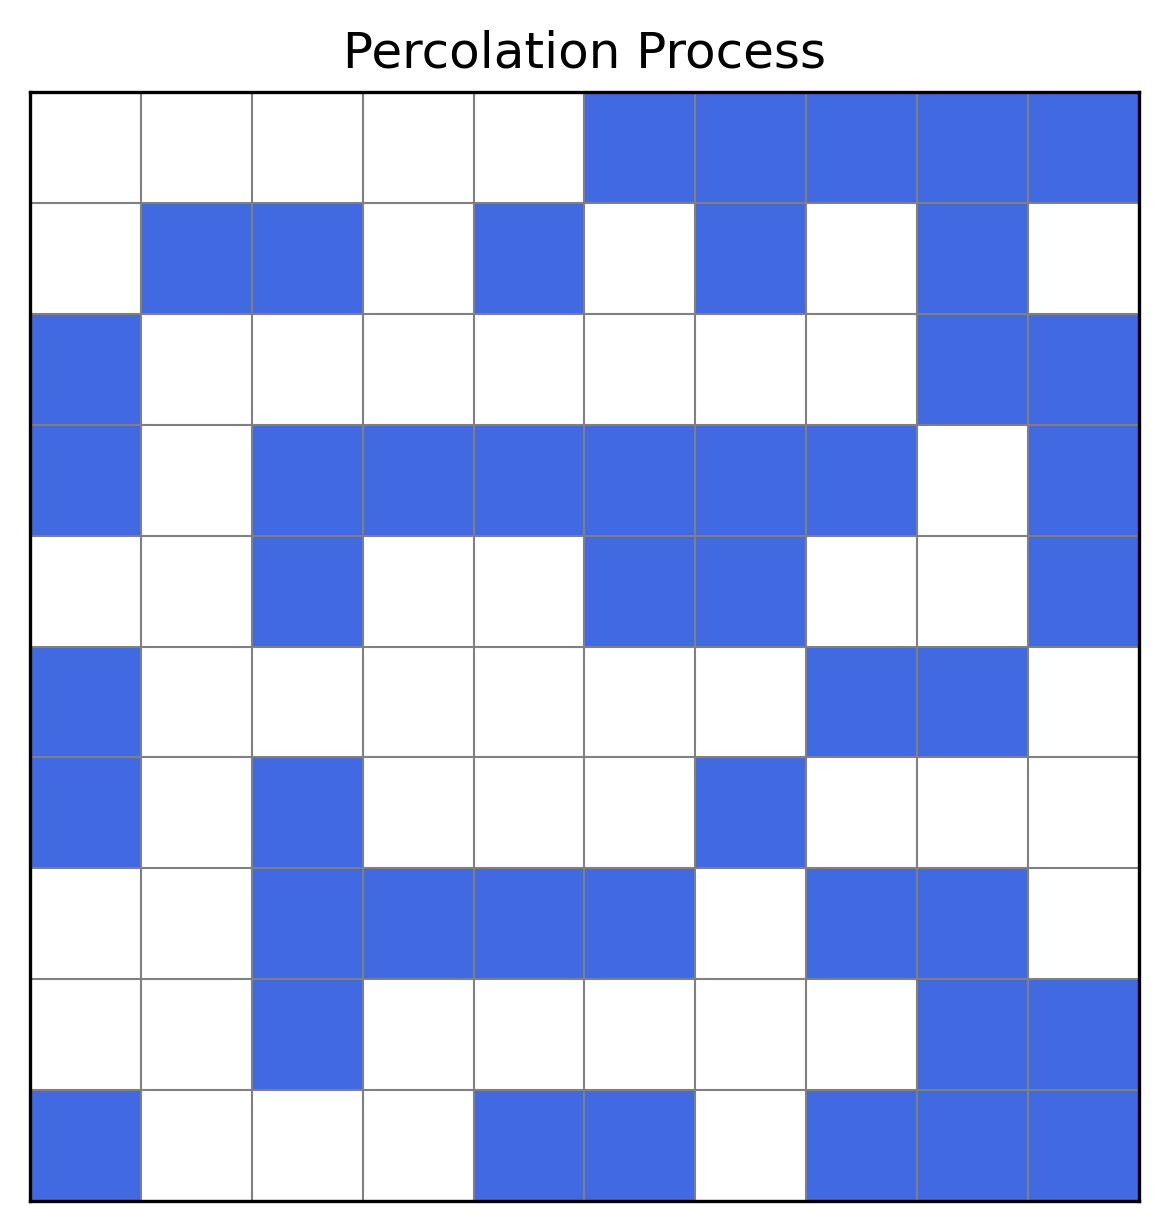
\includegraphics[width=0.75\linewidth]{../figures/percolation1.png}
        \caption{Red cuadrada.}
        \label{fig:subfig1}
    \end{subfigure}
    \hspace{0.02 cm}
    \begin{subfigure}[h]{0.45\textwidth}
        \centering
        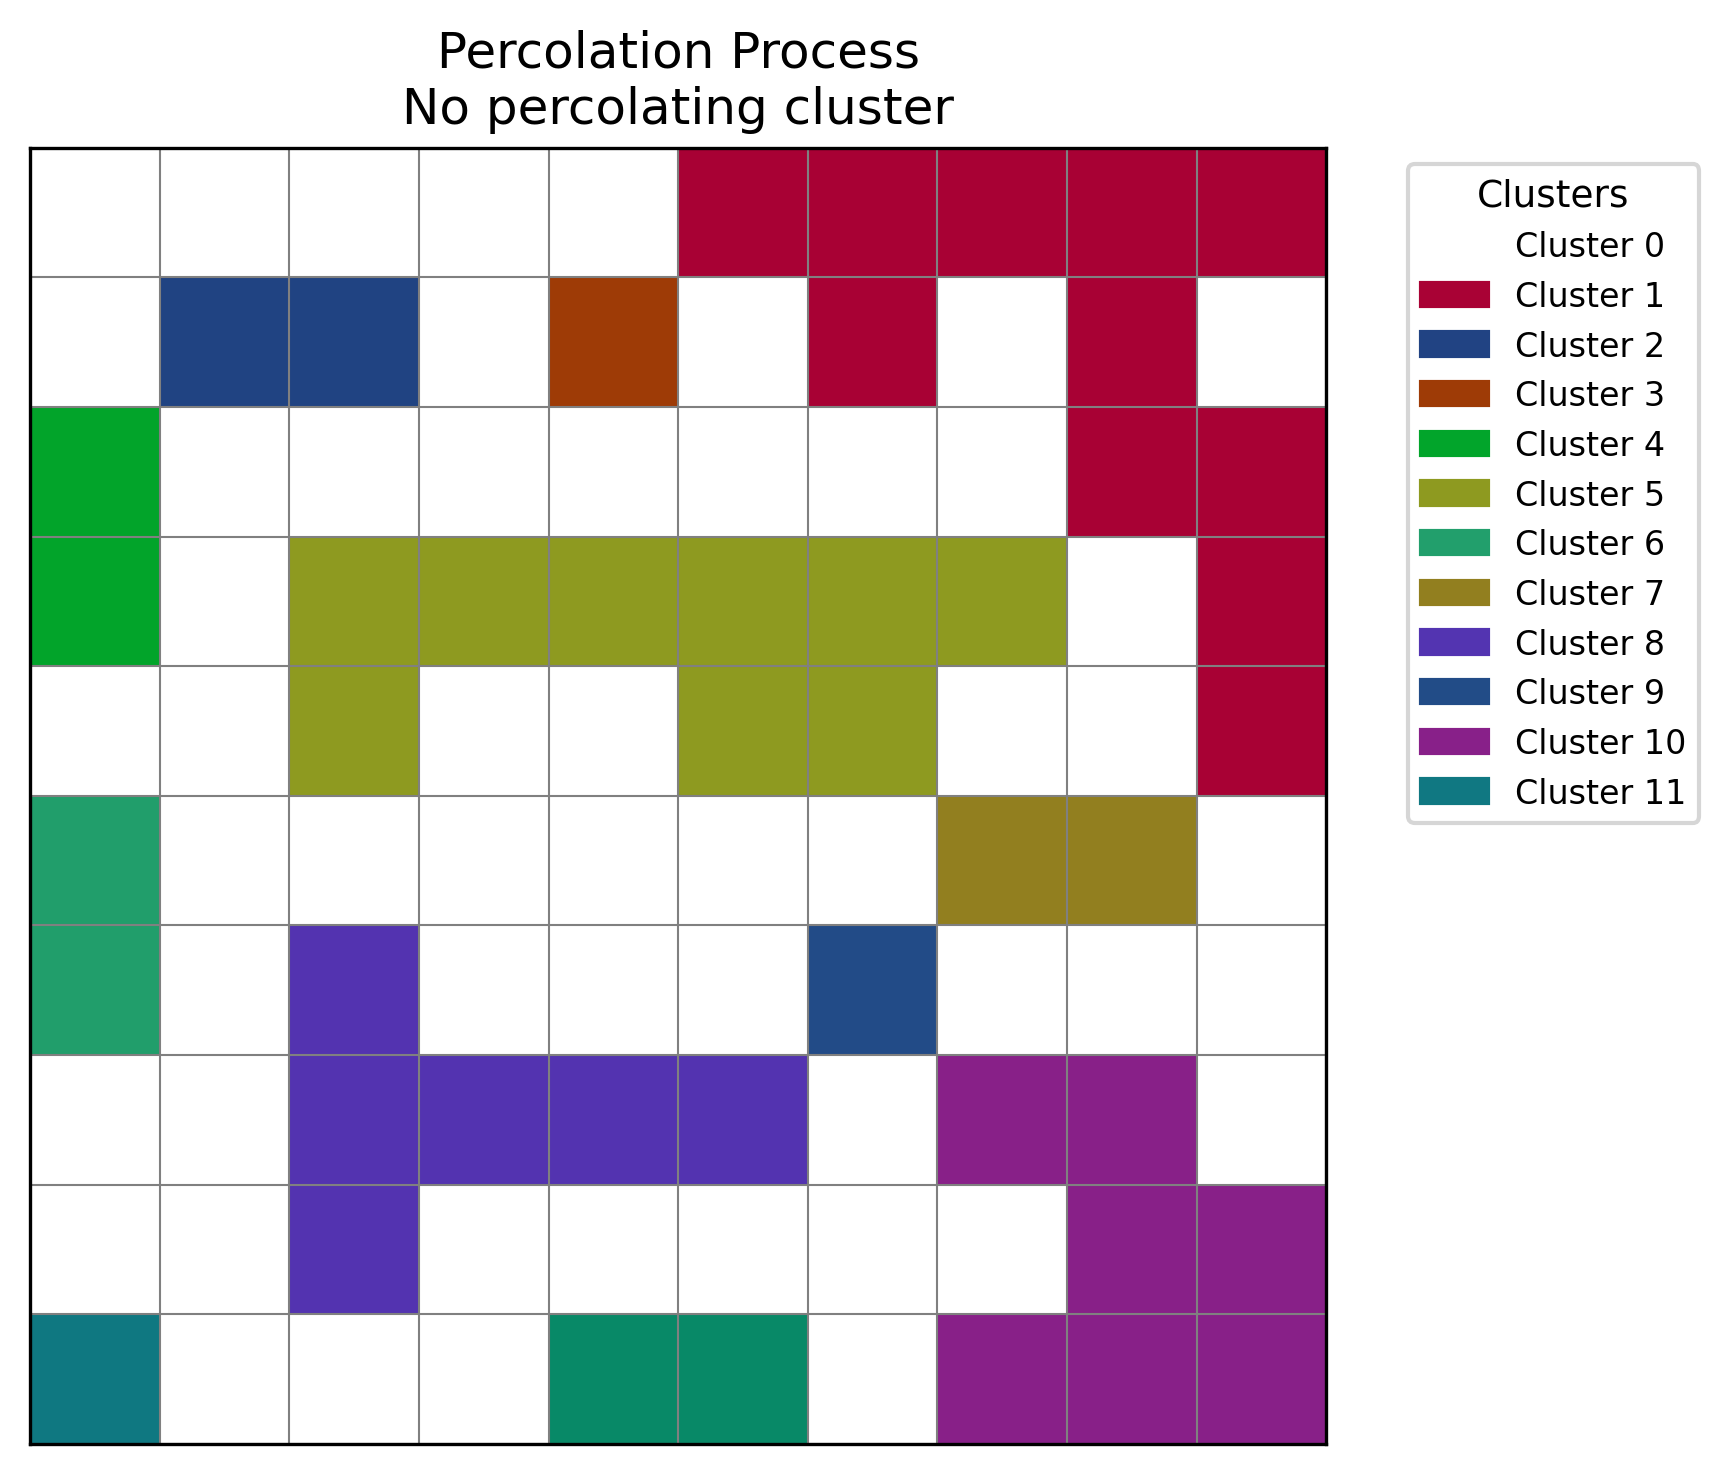
\includegraphics[width=0.9\linewidth]{../figures/clusterpercolation1.png}
        \caption{Clústeres individuales.}
        \label{fig:subfig2}
    \end{subfigure}
    \caption{Proceso de percolación para una red cuadrada por debajo de la probabilidad crítica, \( p = 0.5 \) y \( L = 10 \).}
    \label{fig:1}
\end{figure}

\begin{figure}[H]
    \centering
    \begin{subfigure}[h]{0.4\textwidth}
        \centering
        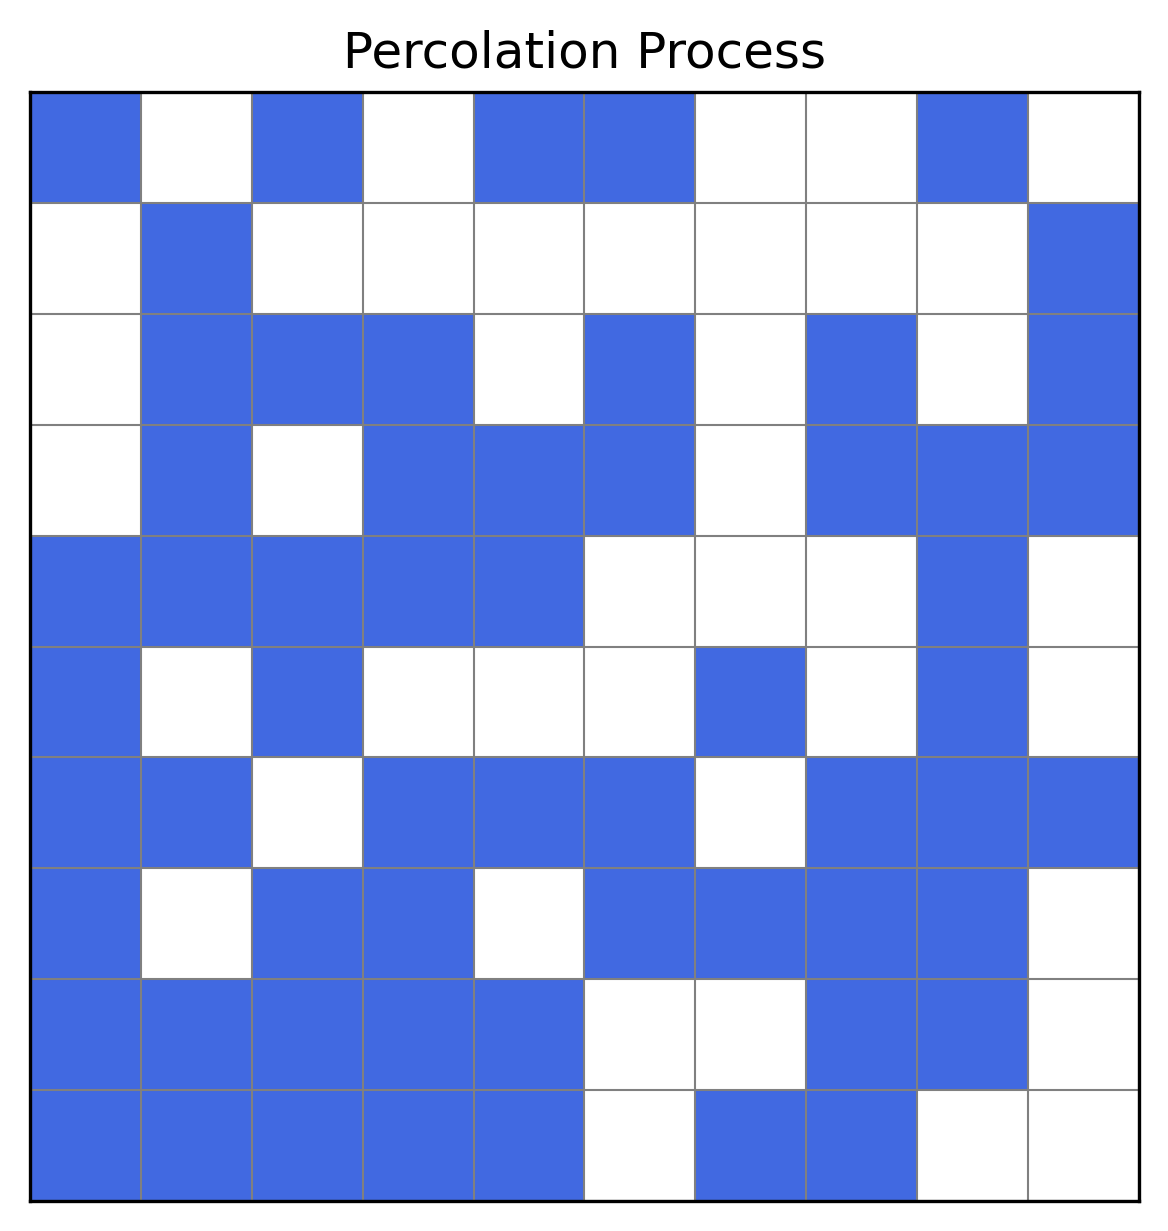
\includegraphics[width=0.75\linewidth]{../figures/percolation2.png}
        \caption{Red cuadrada.}
        \label{fig:subfig3}
    \end{subfigure}
    \hspace{0.02 cm}
    \begin{subfigure}[h]{0.45\textwidth}
        \centering
        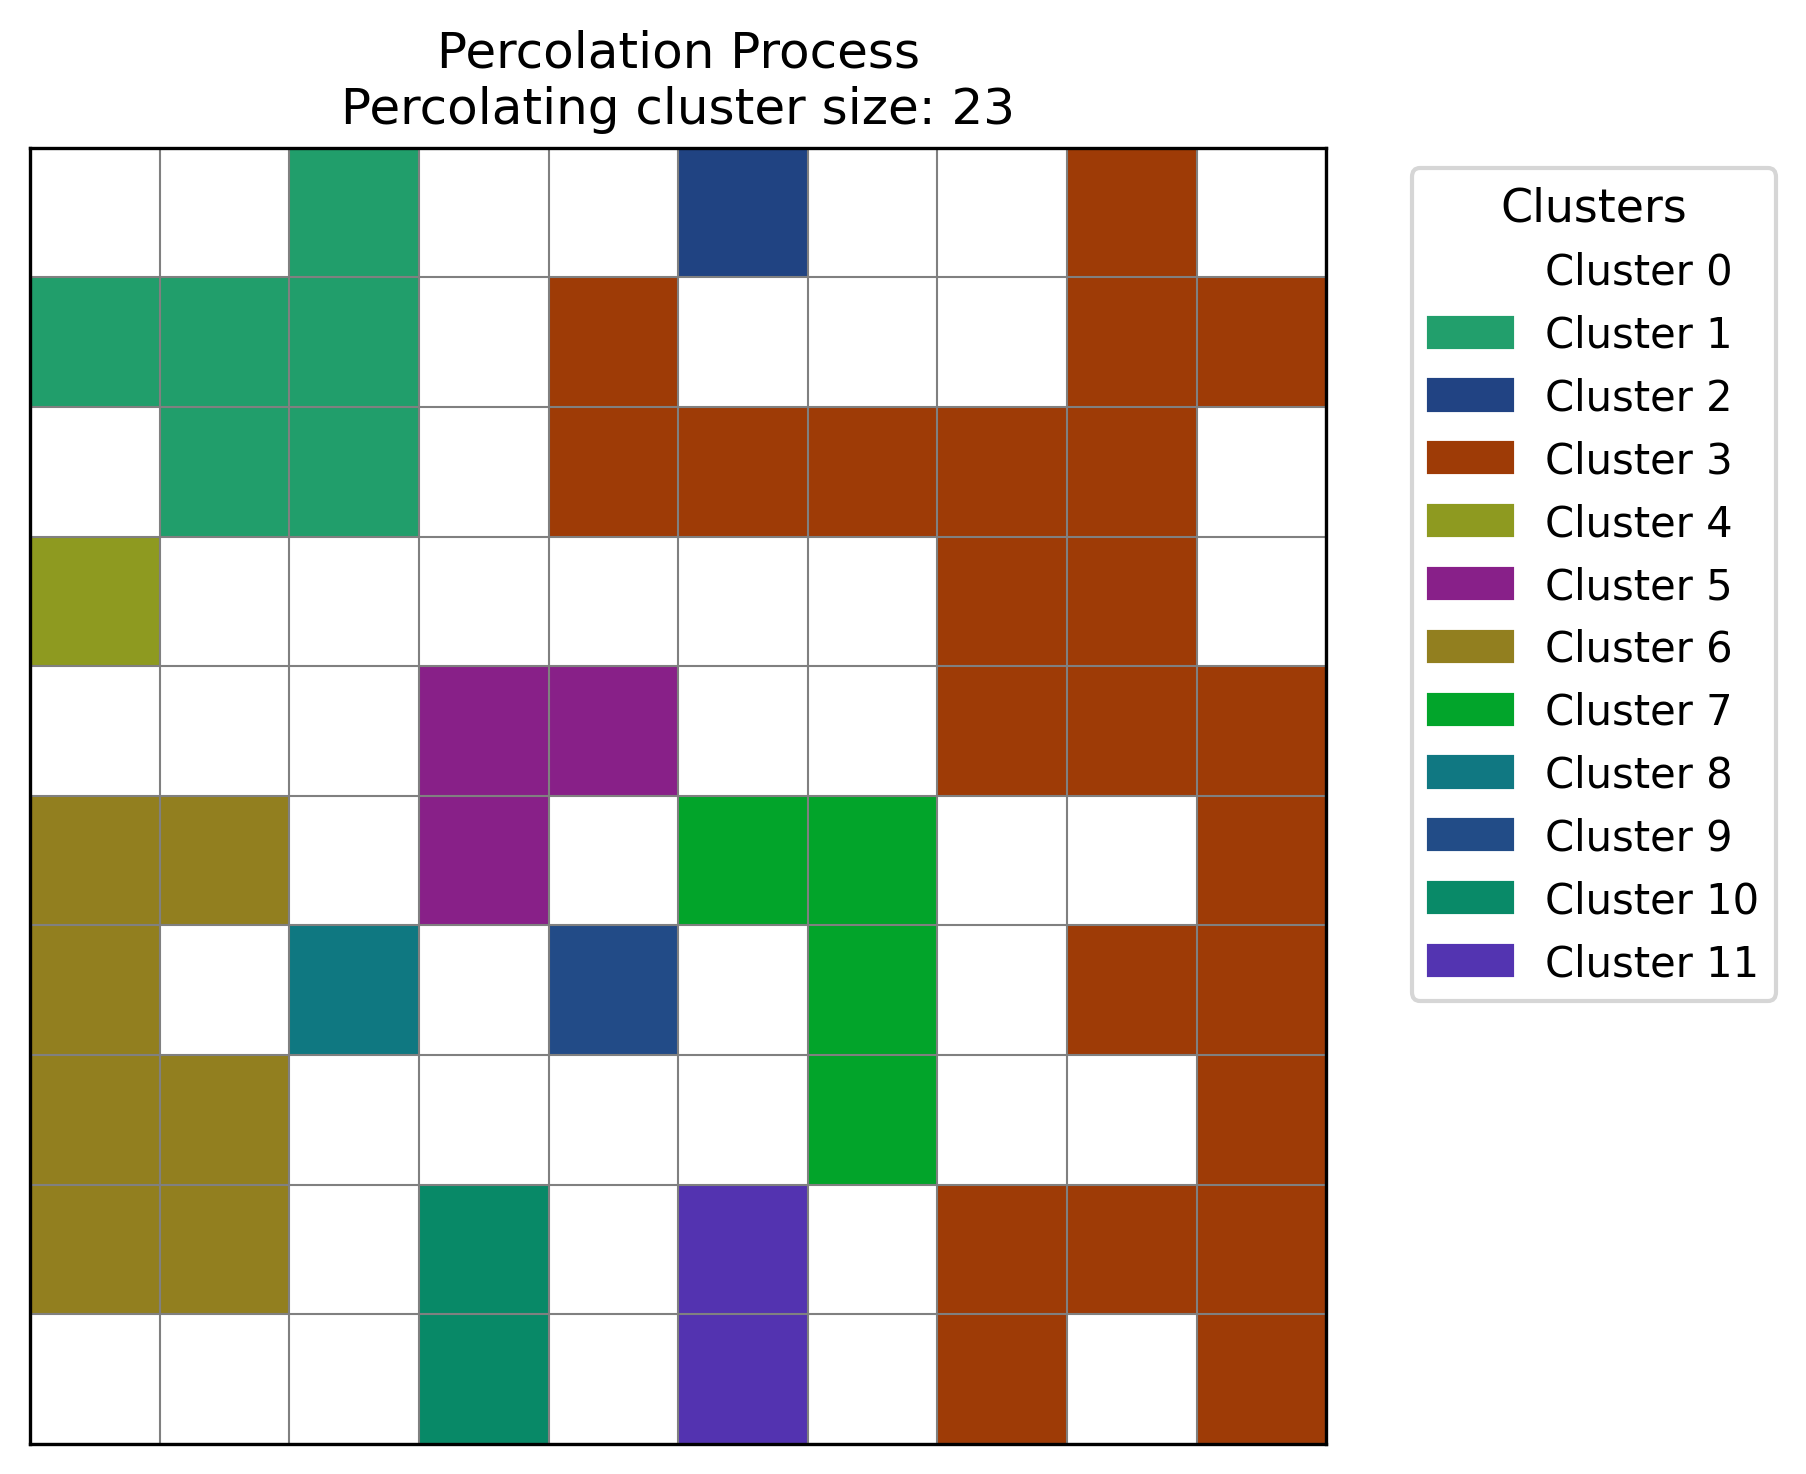
\includegraphics[width=0.9\linewidth]{../figures/clusterpercolation2.png}
        \caption{Clúster percolante.}
        \label{fig:subfig4}
    \end{subfigure}
    \caption{Proceso de percolación para una red cuadrada, \( p = 0.58 \) y \( L = 10 \), donde emerge un clúster percolante.}
    \label{fig:2}
\end{figure}

En este sentido, los objetivos específicos de este proyecto son calcular la probabilidad de percolación \( P(p, L) \), es decir, la fracción de configuraciones con un clúster que conecta lados opuestos (vertical u horizontalmente), analizar el tamaño promedio del clúster más grande \( s(p, L) \) en función de \( p \) y \( L \) y evaluar el impacto del nivel de optimización e implementación de simulaciones computacionales en el tiempo de cómputo para distintos \( L \).
\\

Así, dado el carácter probabilístico del modelo, las simulaciones se repiten múltiples veces para cada combinación de \( p \), \( L \) y nivel de optimización, permitiendo estimar promedios y desviaciones estándar. Computacionalmente, el código se implementó en C++ con estructura modular, usando un \texttt{Makefile} para automatizar ejecución, análisis de desempeño, pruebas unitarias y perfilamiento, como se detalla en la metodología.


\section{Metodología}
Para realizar las simulaciones se trabajo con el programa contenido en el repositorio $\texttt{Percolation\_2025\_I\_IntroSciCompHPC}$ \cite{Mayorga2024} en su rama $\texttt{master}$ cuya estructura es 

\begin{verbatim}
.Percolation_2025_I_IntroSciCompHPC
|__ .github
|   |__ workflows
|__ .vscode
|__ figures
|__ include
|__ profiling
|__ src
|   |__ resultados
|__ Makefile
\end{verbatim}

tal que en $\texttt{figures}$ se encuentran tanto las figuras utilizadas en este trabajo como los códigos necesarios para realizarlas, en $\texttt{include}$ se encuentran las implementaciones de funciones y librerías necesarias para llevar a cabo las simulaciones, teniéndose $\texttt{catch2}$, $\texttt{hoshen\_kopelman.h}$, $\texttt{matrix.h}$, $\texttt{probvalues.h}$ y $\texttt{union\_find.h}$, en $\texttt{profiling}$ se encuentra el flat profile de la simulación del sistema para $L$ = 128 y $p$ = 0.59271 $\texttt{profiling-report.txt}$.
\\

Por otro lado, en $\texttt{src}$ se encuentran los programas:

\begin{itemize}
    \item $\texttt{hoshen\_kopelman.cpp}$: Contiene la función $\texttt{hoshen\_kopelman}$ que permitirá identificar los clústeres en una red bidimensional y la función $\texttt{print\_clusters}$ que permitirá obtener como salida la red bidimensional con los clústeres identificados en, por ejemplo, un archivo.txt.
    \item $\texttt{matrix.cpp }$: Contiene la función $\texttt{generatematrix}$ que generara aleatoriamente mediante la semilla $\texttt{seed}$ una red bidimensional dada la dimensión $L$ y la probabilidad $p$, estos argumentos se pueden recibir por linea de comandos pero en caso de no pasar $\texttt{seed}$, se tomara de forma predeterminada como un número aleatorio mediante $\texttt{std::random\_device}$, tambien contiene a $\texttt{printmatrix}$ que permitirá obtener la salida de la red bidimensional como una matriz. 
    \item $\texttt{probvalues.cpp}$: Contiene la función $\texttt{generate\_p\_values}$ que permitirá generar $N$ valores para $p$ en el intervalo [0, 1] garantizando la existencia de minimo 10 en el intervalo [0.55, 0.65].
    \item $\texttt{script.sh}$: Este script en $\texttt{bash}$ llevara a cabo la simulación para obtener los datos necesarios para encontrar $P(p,L)$ y $s(p,L)$.
    \item $\texttt{printvalues.cpp}$: Permite obtener la salida de $\texttt{generate\_p\_values(N)}$ en, por ejemplo, un archivo .txt.
    \item $\texttt{report.tex}$: Archivo .tex que contiene el reporte en \LaTeX.
    \item $\texttt{report.bib}$: Bibliografia para $\text{report.tex}$
    \item $\texttt{resultados/resumen.csv}$: Archivo .csv con un resumen de los datos obtenidos por medio de $\texttt{script.sh}$.
    \item $\texttt{test.cpp}$: Función main adaptada para realizar distintos tests con $\texttt{Catch2}$.
    \item $\texttt{union\_find.cpp}$: Contiene las funciones $\texttt{UnionFind}$, $\texttt{find}$ y $\texttt{unite}$ que se utilizaran en la función $\texttt{hoshen\_kopelman}$.
    \item $\texttt{main.cpp }$: Función main, recibe como entrada la dimensión de la matriz $L$, la probabilidad $p$ y de forma opcional la semilla $\texttt{seed}$ para el llenado aleatorio por medio de $\texttt{generatematrix}$, realiza la clasificación de los clusters por medio de $\texttt{hoshen\_kopelman}$ e imprime la matriz sin clasificar, la matriz con los clústeres clasificados, si hay percolación y en dado caso el tamaño del clúster percolante.
    \item $\texttt{time\_main.cpp}$ Función main para calcular los tiempos de Wall y CPU para la función $\texttt{main}$ por medio de la libreria $\texttt{chrono}$ y $\texttt{ctime}$.
\end{itemize}

Finalmente, mediante el archivo $\texttt{Makefile}$ se automatizan todos los procesos descritos anteriormente.

\subsection{Algoritmo HK}
El algoritmo de Hoshen-Kopelman (HK), descrito originalmente por Joseph Hoshen y Raoul Kopelman en 1976 , es un método computacionalmente eficiente para identificar y etiquetar clústeres o componentes conectados en una cuadrícula o red. Su diseño está optimizado para minimizar el número de comparaciones necesarias, lo que lo hace particularmente adecuado para el análisis de fenómenos de percolación \cite{OntosightAINd}.

\begin{enumerate}[label=\textbf{\arabic*)}, ref=\arabic*)]
    \item \textbf{Inicialización del proceso}\\
    La función \texttt{hoshen\_kopelman} recibe como entrada una matriz que representa una cuadrícula, donde los valores, usualmente ceros y unos, indican si un sitio está vacío u ocupado, respectivamente. También recibe el tamaño lateral de la cuadrícula, L. Se crea un vector $\texttt{labels}$ del mismo tamaño que la matriz, inicializado con ceros, para almacenar las etiquetas de los clústeres; un 0 en $\texttt{labels}$ significa que la celda está vacía o aún no ha sido etiquetada. Se inicializa una estructura $\texttt{UnionFind}$ ($\texttt{uf}$) con un tamaño N+1 (siendo N = L*L), la cual es esencial para manejar la equivalencia entre las etiquetas de los clústeres. Finalmente, $\texttt{next\_label}$ se establece en 1, marcando la primera etiqueta disponible para asignar a un nuevo clúster.
    
    \begin{enumerate}[label=\textbf{\roman*)}, ref=\roman*)]
        \item \textbf{Estructura $\texttt{UnionFind}$:} La estructura $\texttt{UnionFind}$ es fundamental para la eficiencia del algoritmo, permitiendo la gestión de conjuntos disjuntos. Se compone de un vector $\texttt{parent}$, donde $\texttt{parent[i]}$ almacena el padre del elemento i; inicialmente, cada elemento es su propio padre. El método $\texttt{find(x)}$ localiza la raíz del conjunto al que pertenece x, optimizando las búsquedas futuras mediante la compresión de caminos, lo que hace que los nodos apunten directamente a la raíz. El método $\texttt{unite(x,y)}$ fusiona los conjuntos que contienen a x e y. Para ello, encuentra las raíces de x e y, y si estas son diferentes, establece la raíz de uno como padre de la raíz del otro, logrando así la unión de los dos conjuntos.
    \end{enumerate}
    \item \textbf{Etiquetado preliminar (Primera pasada)}\\
    El algoritmo recorre cada celda de la matriz. Para cada celda (i, j) que se encuentra ocupada,es decir, $\texttt{matrix[id] == 1)}$, se examinan sus vecinos adyacentes: "norte" (up) y $"$oeste" (left). Si ambos vecinos están vacíos o no ocupados, se le asigna una nueva etiqueta a la celda actual $\texttt{(labels[id] = next\_label++)}$. Si solo el vecino Norte está ocupado, la celda actual hereda la etiqueta de su vecino Norte $\texttt{(labels[id] = up)}$. De manera similar, si solo el vecino Oeste está ocupado, la celda actual recibe la etiqueta de su vecino Oeste $\texttt{(labels[id] = left)}$. Cuando ambos vecinos (Norte y Oeste) están ocupados, la celda actual se etiqueta con la menor de las dos etiquetas de sus vecinos $\texttt{(labels[id] = std::min(up, left))}$. Además, se utiliza la estructura UnionFind para unir las dos etiquetas $\texttt{(uf.unite(up, left))}$, indicando que pertenecen al mismo clúster. Esta unión es crítica porque permite reconocer que dos etiquetas inicialmente distintas forman parte de un mismo clúster.
    \item \textbf{Compactación de etiquetas (Segunda Pasada)}\\
    Después de la primera pasada, es posible que algunas celdas tengan etiquetas diferentes pero pertenezcan al mismo clúster debido a las uniones realizadas por UnionFind. Esta etapa se encarga de $"$compactar$"$ esas etiquetas, asegurando que todos los miembros de un mismo clúster compartan una única etiqueta unificada. Para esto, se emplean dos $\texttt{(unordered\_map): root\_to\_compact}$, que relaciona la $"$raíz" de un clúster obtenida mediante $\texttt{UnionFind::find()}$ con una etiqueta compactada y consecutiva, y $\texttt{cluster\_sizes}$, que almacena el tamaño de cada clúster utilizando estas etiquetas compactadas. El algoritmo itera sobre todas las celdas en labels. Para cada celda que ya ha sido etiquetada, es decir, no es cero, se busca la raíz de su etiqueta utilizando $\texttt{uf.find(labels[i])}$. Si esta raíz aún no ha sido mapeada a una etiqueta compactada, se le asigna una nueva $\texttt{(compact\_label++)}$. Posteriormente, la etiqueta de la celda actual se actualiza a su etiqueta compactada $\texttt{(labels[i] = label)}$, y el tamaño del clúster correspondiente en $\texttt{cluster\_sizes[label]}$ se incrementa.
    \item \textbf{Detección de percolación}\\
    La percolación es un fenómeno que ocurre cuando un clúster logra conectar lados opuestos de la matriz. Para identificar esto, se crean cuatro conjuntos desordenados $\texttt{(unordered\_set)}$ que almacenan las etiquetas de los clústeres que tocan cada uno de los cuatro bordes de la matriz: top (fila superior), bottom (fila inferior), left (columna izquierda), y right (columna derecha). Se recorren las celdas de estas filas y columnas específicas, insertando las etiquetas de las celdas ocupadas en sus respectivos conjuntos.
\\

Para la percolación vertical, se verifica si alguna etiqueta está presente tanto en el conjunto top como en el conjunto bottom. Si se encuentra una etiqueta común, indica la existencia de un clúster que conecta la parte superior e inferior de la matriz. De manera similar, para la percolación horizontal, se comprueba si alguna etiqueta existe tanto en el conjunto left como en el conjunto right. Si es así, significa que un clúster conecta el lado izquierdo con el derecho de la matriz. Un conjunto $\texttt{percolating\_labels}$ almacena las etiquetas de los clústeres que percolan, ya sea vertical u horizontalmente. La variable booleana $\texttt{percolates}$ indica si se ha detectado al menos un clúster percolante. Finalmente, se calcula $\texttt{max\_cluster\_size}$ entre todos los clústeres que percolan.

    \item \textbf{Conclusión del algoritmo}\\
    La función concluye devolviendo una estructura $\texttt{ClusterInfo}$. Esta estructura encapsula los resultados clave del análisis, que incluyen $\texttt{cluster\_sizes}$, un mapa que asocia las etiquetas compactadas con sus respectivos tamaños de clúster, $\texttt{percolates}$, un valor booleano que indica si se produjo percolación, $\texttt{max\_cluster\_size}$ el tamaño del clúster percolante más grande, y $\texttt{labels}$ el vector final de etiquetas compactadas asignadas a cada celda de la matriz.
\end{enumerate}

\subsection{Wall time y CPU time}
\label{WtCPUt}
Con el fin de obtener los Wall time y CPU time para el tiempo de computo de nuestra función $\texttt{main.cpp}$ se utilizo la función $\texttt{time\_main.cpp}$ esta realiza el mismo procedimiento que $\texttt{main.cpp}$, sin embargo, no imprime la salida de la matriz después del llenado y después de la identificación de los clústeres, tal que su unica salida es de la forma $L$, Wall time y CPU time y mediante el comando de $\texttt{GNU Parallel}$

\begin{center}
\verb|parallel './time_mainO{1}.x {3} {2} >> time-{1}-{3}.txt'|\\
\verb|::: 1 3 ::: $(cat probabilidades10.txt) ::: {100..2000..100}'|
\end{center}

se obtienen distintos archivos .txt de la forma $\texttt{time-opt-$L$.txt}$ que permitirán graficar los tiempos de computo para los niveles de optimización $\texttt{-O1}$ y $\texttt{-O3}$. Notese que no hay valor de entrada por la linea de comandos para $\texttt{seed}$, por ende, la salida es aleatoria.


\subsection{Script en bash $\texttt{script.sh}$}

El script en bash automatiza la ejecución de simulaciones de percolación para distintos tamaños de red y probabilidades, utilizando un programa ejecutable llamado $\texttt{main.x}$. Al iniciar, elimina cualquier carpeta de resultados previa y crea una nueva estructura de directorios para almacenar datos crudos, archivos auxiliares y gráficos. Luego, define una lista de tamaños de red $L$ que serán evaluados y genera todas las combinaciones posibles con los valores de probabilidad listados en el archivo $\texttt{probabilidades50.txt}$, es decir, mediante 50 probabilidades distintas obtenidas mediante $\texttt{probvalues.cpp}$. Estas combinaciones se almacenan en un archivo temporal para su procesamiento posterior.\\
 
El núcleo del script es una función llamada $\texttt{simulate}$, que toma como entrada un valor de $L$ y una probabilidad $p$. Para cada combinación, ejecuta 10 bloques de 10 repeticiones del programa principal, recolectando el tamaño del mayor clúster percolante y si ocurrió o no percolación en cada ejecución. Con esta información, calcula el valor medio de la probabilidad de percolación $P(p,L)$ y el tamaño promedio del clúster percolante $s(p,L)$ normalizado respecto al área de la red, junto con sus respectivas desviaciones estándar. Los resultados se guardan en archivos individuales para cada combinación y también se imprimen en formato $\texttt{.csv}$ como una línea resumen disponible para el usuario en caso de desear ver la salida de datos especifica. Cabe mencionar que, como se pudo inferir, la entrada de la semilla $\texttt{seed}$ por la linea de comandos es nula, se considera que dado que se realizan por cada valor de probabilidad $p$ 100 iteraciones y se itera 50 veces por tamaño, la magnitud del tamaño de los datos utilizados es lo suficientemente grande como para permitir un muestreo estadístico solido y confiable sin importar la generación de estos, es decir, los resultados son absolutamente reproducibles a pesar de la aleatoriedad de la semilla.\\

Finalmente, el script utiliza $\texttt{GNU parallel}$ para ejecutar múltiples simulaciones de forma concurrente, acelerando considerablemente el proceso. Una vez completadas todas las combinaciones, se genera un archivo $\texttt{resumen.csv}$ que contiene los resultados ordenados por tamaño de red y probabilidad. Finalmente, se limpian los archivos temporales utilizados durante la ejecución y se ordenan los archivos de resultados finales para facilitar su análisis posterior

\subsection{Código para gráficar}
Para gráficar las matrices llenadas como las matrices con los clústeres identificados se utilizaron los codigos $\texttt{visualization.cpp}$ y $\texttt{clustervisualization.cpp}$ que permiten la salida en archivos.txt de las matrices obtenidas y controlar la dimensión $L$, la probabilidad $p$ y la semilla $\texttt{seed}$ con el fin de obtener gráficas reproducibles. De esta manera, mediante los scripts de $\texttt{python}$ $\texttt{visualize.py}$ y $\texttt{clustervisualize.py}$ reciben las matrices, por ejemplo, de la forma: 
\\

\begin{lstlisting}[style=bash-style]
./figures/visualization.x 10 0.5 0.6 > figures/data1.txt
./figures/visualization.x 10 0.58 15 > figures/data2.txt
python3 ./figures/visualize.py
./figures/clustervisualization.x 10 0.5 0.6 > figures/data_clusters1.txt
./figures/clustervisualization.x 10 0.58 15 > figures/data_clusters2.txt 
./figures/clustervisualization.x 500 0.55 0.6 > figures/data_clusters3.txt
./figures/clustervisualization.x 500 0.595 0.6 > figures/data_clusters4.txt
python3 ./figures/clustervisualize.py
\end{lstlisting}

De esta manera, en el ejemplo presentado, la salida para $\texttt{data1.txt}$ y $\texttt{data\_clusters1.txt}$ junto con la salida para $\texttt{data2.txt}$ y $\texttt{data\_clusters2.txt}$ permiten obtener las figuras \ref{fig:1} y \ref{fig:2}. Por otro lado, la salida de $\texttt{data\_clusters3.txt}$ y $\texttt{data\_clusters4.txt}$ nos permiten obtener las figuras \ref{fig:3a} y \ref{fig:3b}.

\begin{figure}[H]
    \centering
    \begin{subfigure}[h]{0.45\textwidth}
        \centering
        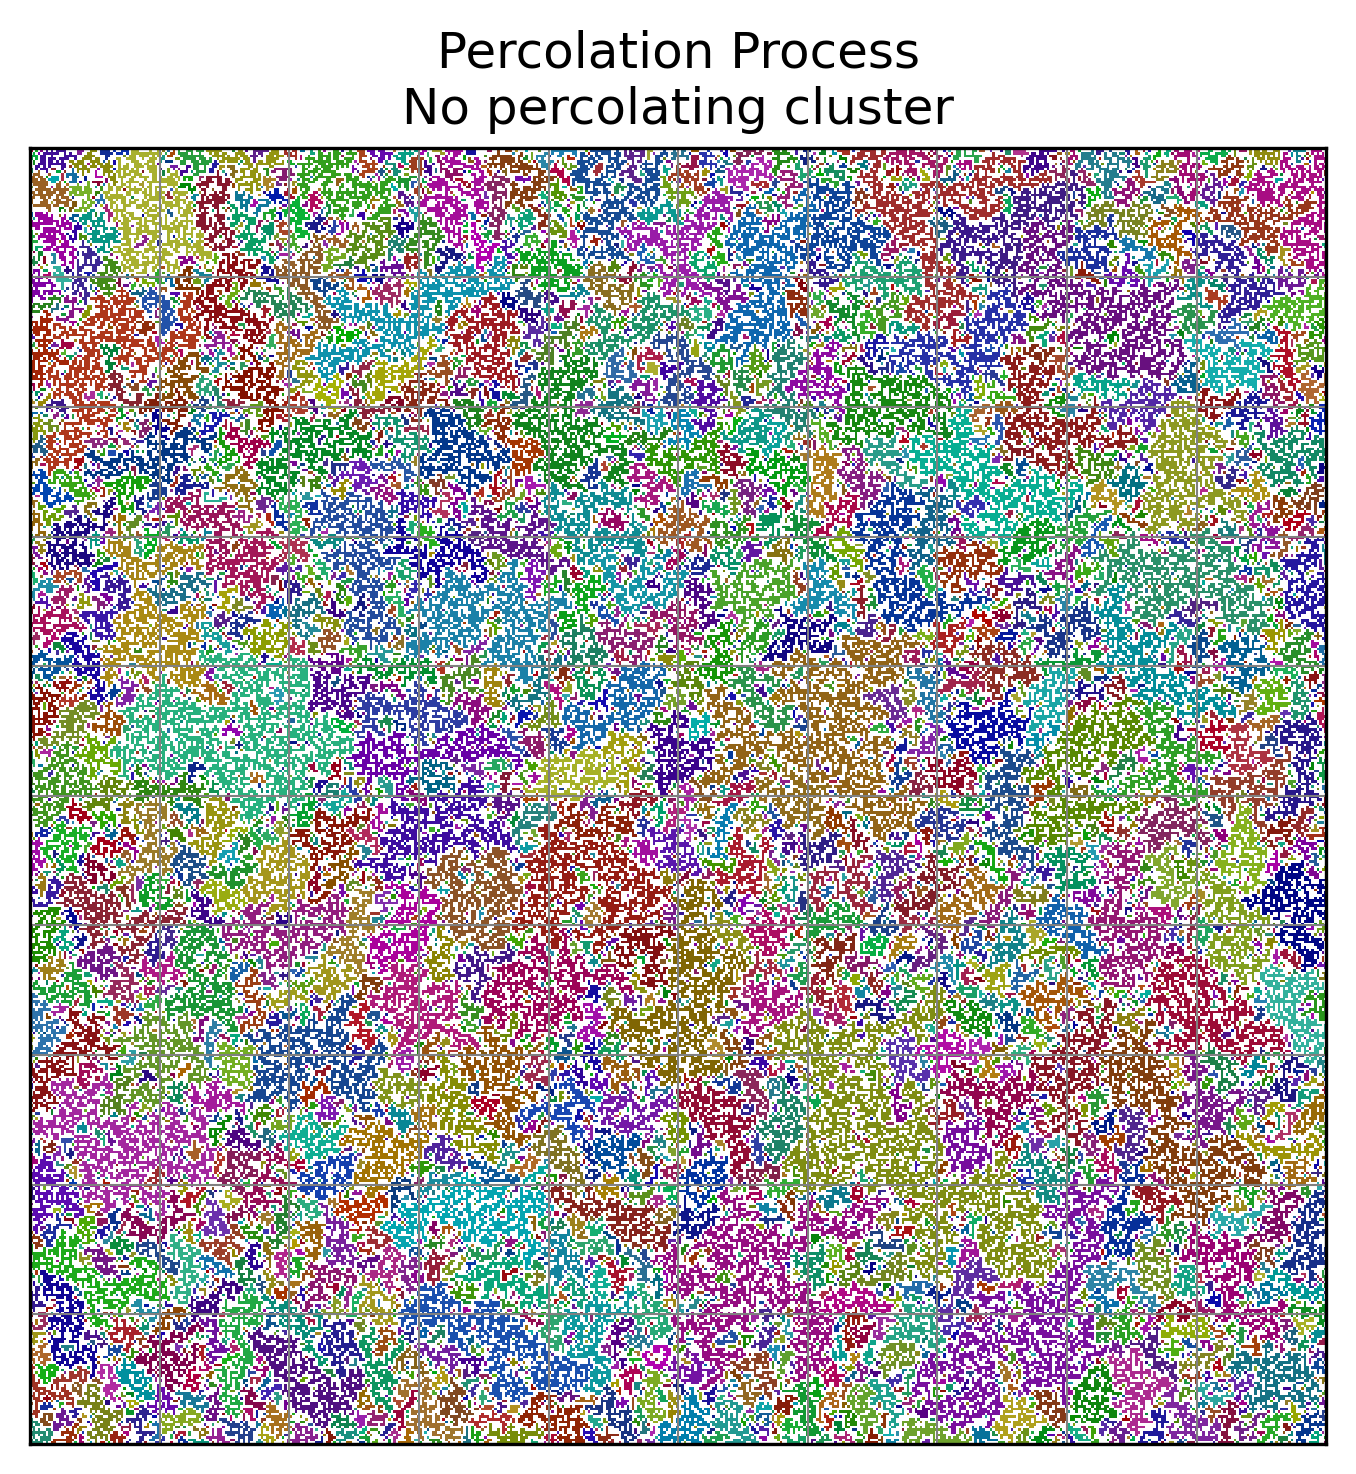
\includegraphics[width=1.0\linewidth]{../figures/clusterpercolation3.png}
        \caption{$p$ = 0.5.}
        \label{fig:3a}
    \end{subfigure}
    \hspace{0.02 cm}
    \begin{subfigure}[h]{0.45\textwidth}
        \centering
        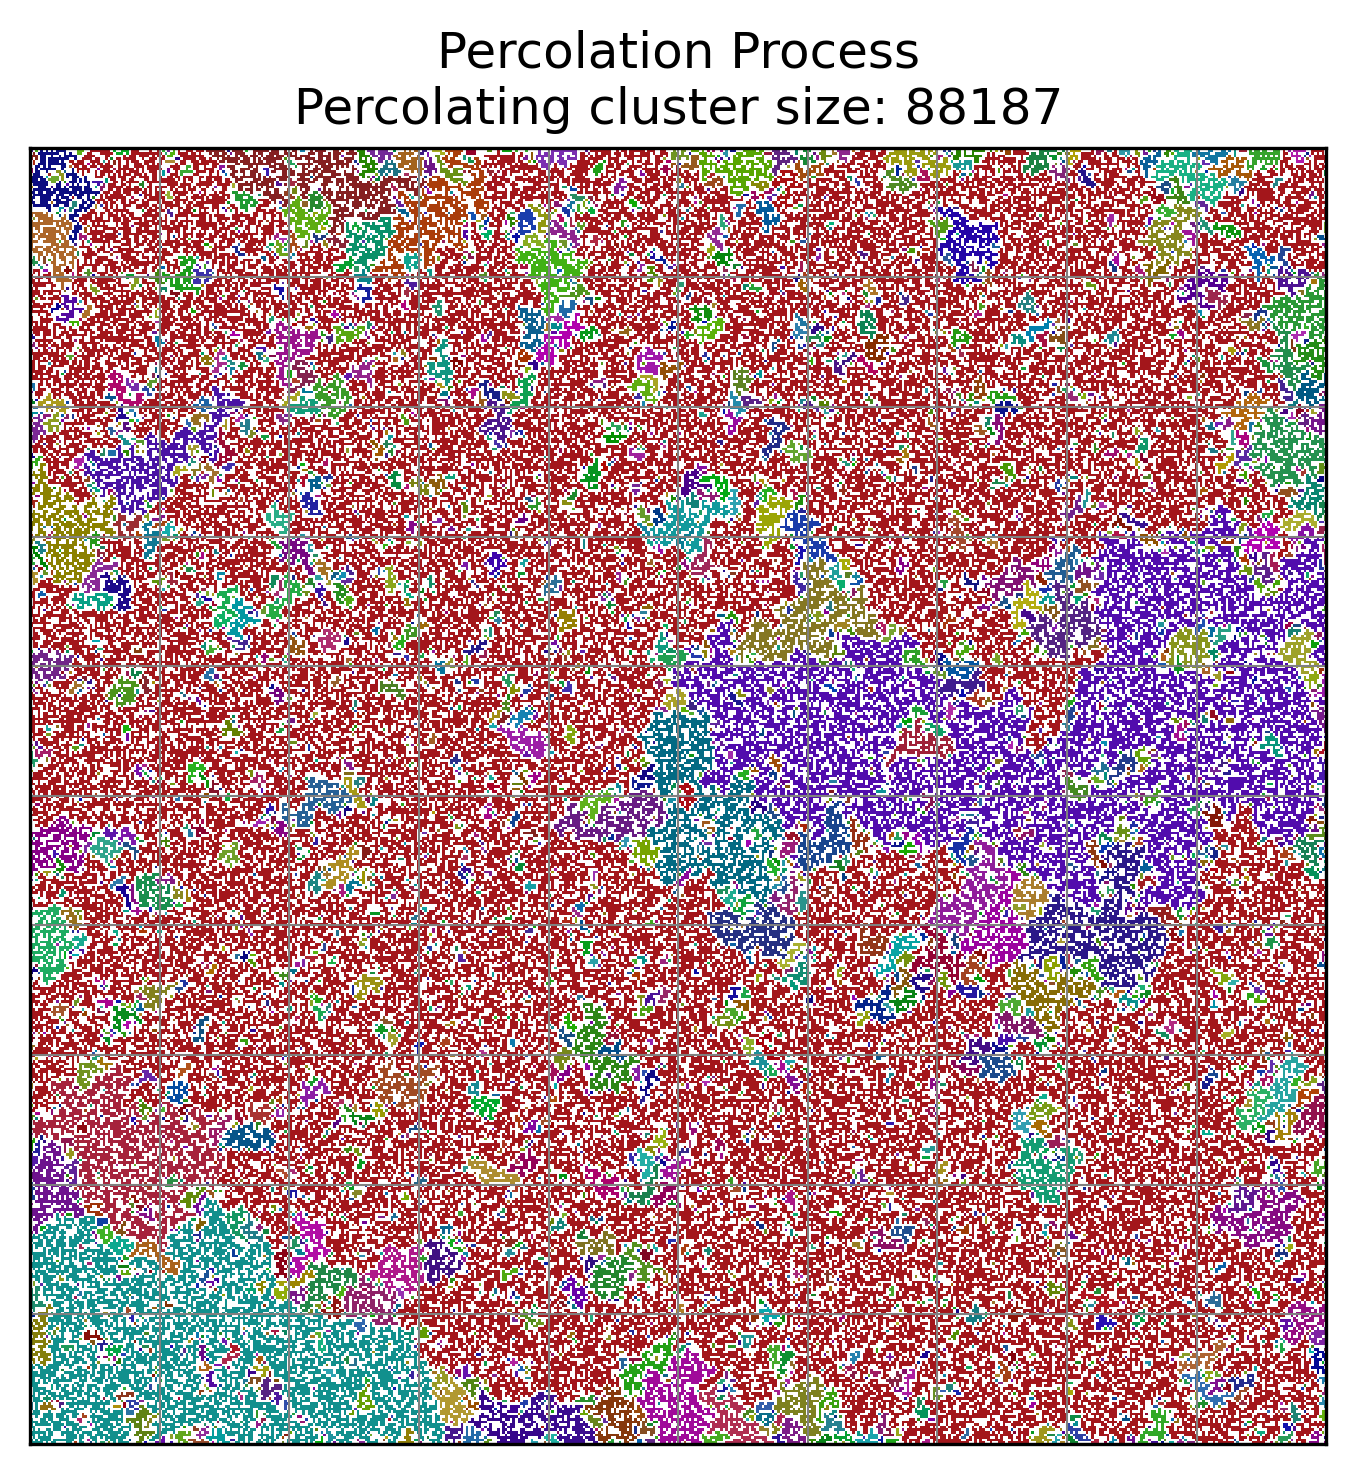
\includegraphics[width=1.0\linewidth]{../figures/clusterpercolation4.png}
        \caption{$p$ = 0.595.}
        \label{fig:3b}
    \end{subfigure}
    \caption{Proceso de percolación para una red cuadrada de dimensiones $L$ = 500.}
    \label{fig:3}
\end{figure}


Por otro lado, el script $\texttt{figures.py}$ permite obtener las gráficas para $P(p,L)$ y $s(p,L)$ gracias a la salida obtenida mediante el script en $\texttt{bash}$ y el script $\texttt{time\_figure.py}$ procesa los archivos de datos temporales generados por las mediciones de rendimiento para diferentes tamaños de matriz $L$ y niveles de optimización. Este script lee los archivos con formato $\texttt{time-opt-L.txt}$, donde $\texttt{opt}$ corresponde al nivel de optimización $\texttt{-O1}$ o $\texttt{-O3}$, y $L$ representa las dimensiones de la matriz.
\\

Para cada combinación de parámetros, el script calcula el promedio y la desviación estándar tanto del Wall time como de CPU time para los tiempos observados para el mismo $L$ en distintos valores de $p$ aleatorios, con el fin de estandarizar el resultado. Los datos se visualizan en una gráfica con escala logarítmica en ambos ejes, donde se pueden comparar los tiempos de ejecución entre los diferentes niveles de optimización. La gráfica resultante incluye:

\begin{itemize}
\item Tiempo de pared representado con marcadores circulares
\item Tiempo de CPU representado con marcadores cuadrados (escalado por un factor de 1000)
\item Líneas sólidas para el nivel de optimización $\texttt{-O1}$
\item Líneas discontinuas para el nivel de optimización $\texttt{-O3}$
\item Barras de error que muestran la desviación estándar
\end{itemize}

\subsection{Automatización por medio de Makefile}
Para automatizar los procesos descritos anteriormente se crearon distintos targets para el archivo $\texttt{Makefile}$ destinados a varias tareas especificas. Los mas relevantes para el programa y que no son subdependencias de otro target son:

\begin{itemize}

\item \texttt{make simul}: Compila y ejecuta una simulación rápida con parámetros predeterminados ($L$=4, $p$=0.6, $\texttt{seed}$=10). Útil para verificar que el código funciona correctamente.

\item \texttt{make test}: Ejecuta pruebas unitarias utilizando la librería \texttt{Catch2}. Puede filtrar pruebas específicas usando \texttt{FILTER=...}.

\item \texttt{make report}: Compila el documento LaTeX del reporte, procesa la bibliografía si existe, y genera un PDF final. Verifica que todas las figuras necesarias estén presentes antes de compilar.

\item \texttt{make profile}: Realiza un análisis de rendimiento completo, incluyendo:
\begin{itemize}
    \item Flat profile con \texttt{gprof} (guardado en \texttt{profiling/analysis.txt})
    \item Flame graph con \texttt{perf} (guardado como \texttt{profiling/flamegraph.svg})
\end{itemize}
Usa parámetros de prueba ($L$=8, $p$=0.5, $\texttt{seed}$=10).

\item \texttt{make debug}: Compila el programa con flags de depuración y lo ejecuta bajo GDB para facilitar la identificación de errores.

\item \texttt{make valgrind}: Realiza un análisis de memoria con Valgrind para detectar leaks y accesos inválidos, usando parámetros de prueba ($L$=6, $p$=0.6, $\texttt{seed}$=10).

\item \texttt{make clean}: Elimina todos los archivos temporales, ejecutables, datos de cobertura y resultados de profiling. No afecta las figuras ni el reporte final.

\item \texttt{make profiling-report.txt}: Genera un flat profile detallado usando \texttt{perf} para el caso crítico ($L$=128, $p$=0.59271, $\texttt{seed}$=10).

\item \texttt{make run-simulation}: Ejecuta la simulación completa generando todos los archivos de datos necesarios para las gráficas, pero sin generar las figuras.

\item \texttt{make figures}: Genera todas las figuras del análisis, incluyendo:
\begin{itemize}
    \item Gráficas de probabilidad de percolación y tamaño de clústers
    \item Visualizaciones de mallas de ejemplo
    \item Análisis de tiempos de ejecución
\end{itemize}
Requiere que los datos de simulación ya estén generados.

\item \texttt{make clean-figures}: Elimina todas las figuras generadas, permitiendo forzar su regeneración.

\item \texttt{make check-figures}: Verifica si todas las figuras necesarias existen, y si no, las genera automáticamente.

\item \texttt{make help}: Muestra los distintos targets y su uso.

\end{itemize}

\section{Resultados}

\subsection{Figura para el tiempo de computo en función del tamaño del sistema}
Después de realizar el proceso descrito en la sección \ref{WtCPUt} y ejecutar el script $\texttt{time\_figure.py}$ se obtuvo la gráfica presentada en la figura \ref{fig:4}.

\begin{figure}[H]
    \centering
    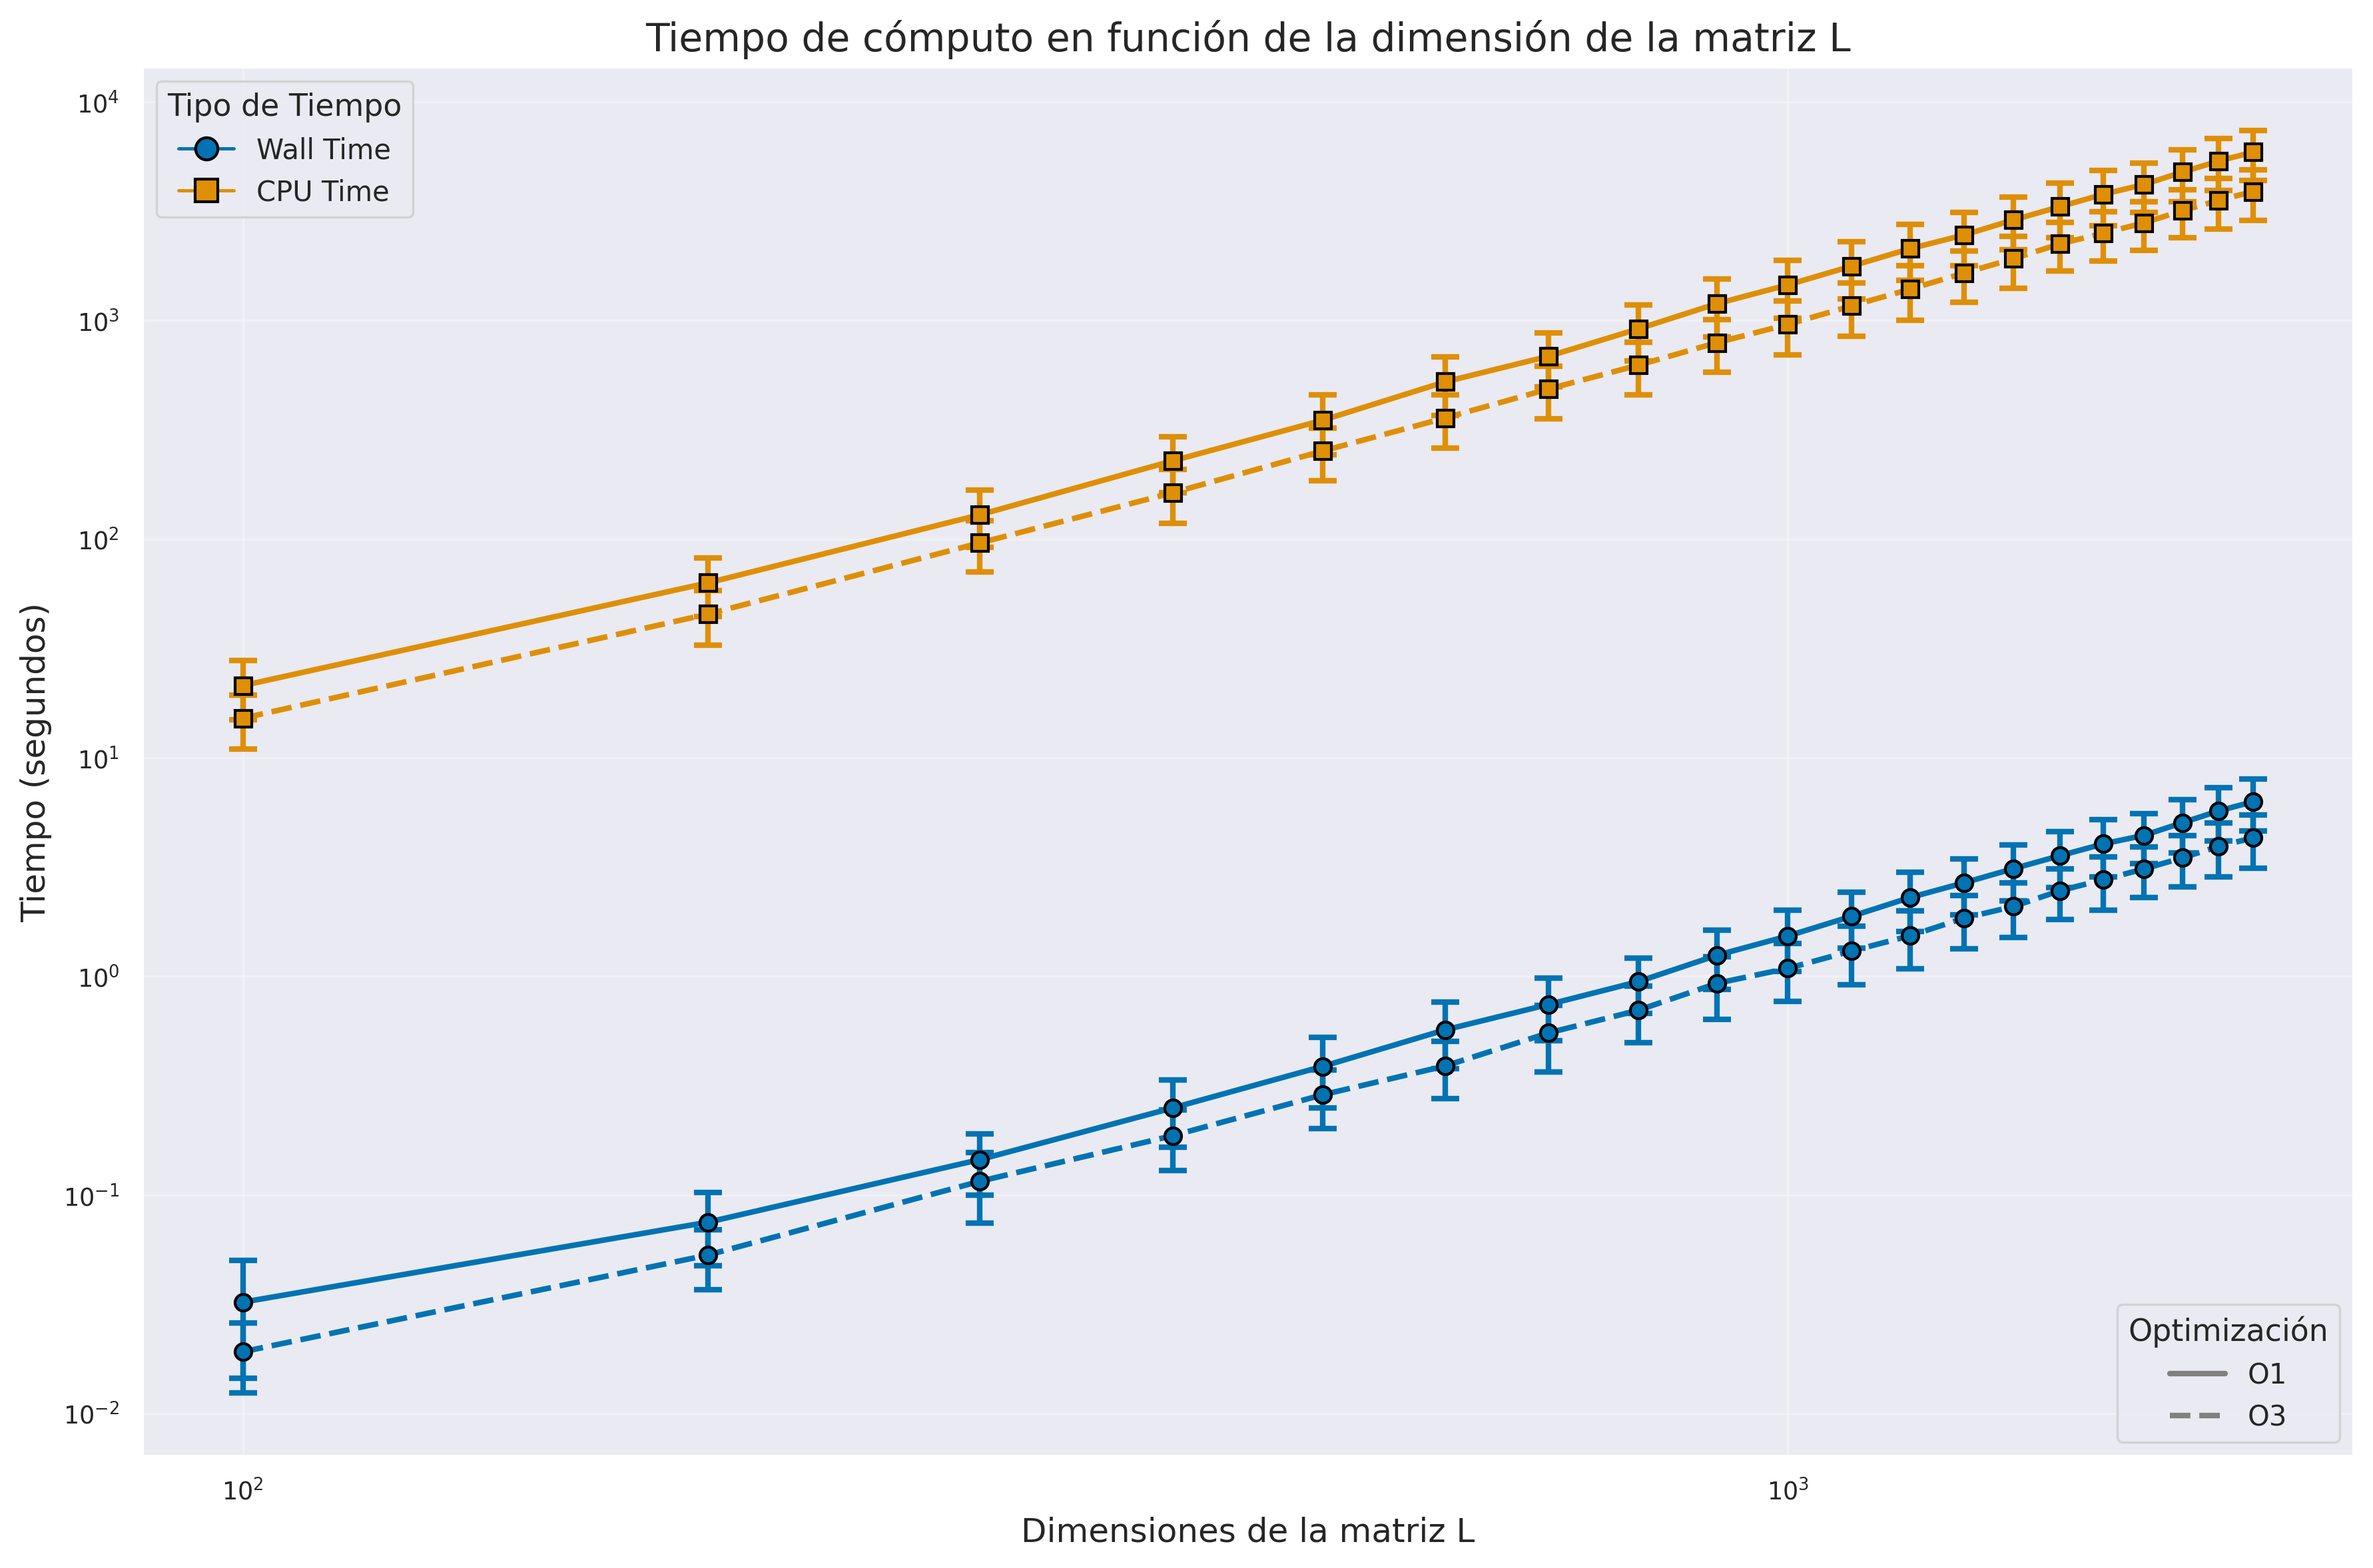
\includegraphics[width=1.0\linewidth]{../figures/time_analysis.png}
    \caption{Tiempos de computo, Wall time y CPU time en función de la dimensión $L$ de la red bidimensional para los niveles de optimización $\texttt{-O1}$ y  $\texttt{-O3}$.}
    \label{fig:4}
\end{figure}

Como se observa, el tiempo de CPU es relativamente mayor al tiempo de Wall debido al uso de $\texttt{GNU Parallel}$, ademas, también se encuentra una mínima diferencia para ambos niveles de optimización, siendo $\texttt{-O3}$ mas rápido. Por estos motivos, para el ejecutable de la función $\texttt{main.cpp}$ se decidió utilizar la bandera de optimización $\texttt{-O3}$ para su compilación y su futura ejecución en las distintas tareas del programa, como, por ejemplo, su aplicación en el script en bash.


\subsection{Optimización por medio del flat profile}

Después de obtener el flat profile mediante $\texttt{perf}$ con el target $\texttt{make profiling-report.txt}$ para el caso crítico, se obtuvo el reporte $\texttt{profiling-report.txt}$.
\\

En este, se realizaron 76 muestras del evento $\texttt{cycles:Pu}$ que corresponde a ciclos de CPU, 64927805 ciclos totales sin tener muestras perdidas obteniendose datos completos. Así, para una sola simulación el tiempo de programa fue del 82.36\% para la función $\texttt{main}$ repartiendose de la forma

\begin{itemize}
    \item 54.77\% para la función $\texttt{hoshen\_kopelman}$, donde las funciones mas costosas son $\texttt{std::unordered\_map::operator[]}$ con un 27.69\% debido al acceso e inserción en $\texttt{hash map}$ y $\texttt{std::unordered\_map::find}$ con un 13.16\% debido a la búsqueda en $\texttt{hash map}$.
    \item 22.86\% para la función $\texttt{generatematrix}$ donde 21.36\% se destino a\\ $\texttt{std::uniform\_real\_distribution::operator()}$.
    \item 3.06\% y 1.66\% para las funciones $\texttt{printmatrix}$ y $\texttt{print\_clusters}$ respectivamente.
\end{itemize}

En consecuencia, se observa que los principales cuellos de botella se encuentran en las operaciones de $\texttt{unordered\_map}$, relacionados con el algoritmo HK y en la generación de números aleatorios para el llenado de las matrices. De esta manera, se propuso optimizar el las funciones $\texttt{hoshen\_kopelman}$ y $\texttt{generatematrix}$ para obtener una simulación mas eficiente. Los cambios implementados se encuentran en la rama $\texttt{optimized\_main}$.
\\

Primero, se implemento para $\texttt{generatematrix}$ la función 
\\

\begin{lstlisting}[style=cpp-style]
FastRandom::FastRandom(int seed) : dis(0.0, 1.0) {
    if (seed == -1) {
        std::random_device rd;
        gen.seed(rd());
    } else {
        gen.seed(seed);
    }
}

// Implementacion de fill_vector
void FastRandom::fill_vector(std::vector<double>& vec) {
    for (auto& val : vec) {
        val = dis(gen);
    }
}

// Implementacion de next()
inline double FastRandom::next() {
    return dis(gen);
}
\end{lstlisting}


tal que la función $\texttt{FastRandom}$ esta incluida en 
$\texttt{matrix.h}$,
\\

\begin{lstlisting}[style=cpp-style]
#ifndef MATRIX_H
#define MATRIX_H

#include <vector>
#include <random>
#include <iostream>

class FastRandom {
private:
    std::mt19937 gen;
    std::uniform_real_distribution<double> dis;
    
public:
    FastRandom(int seed = -1);
    void fill_vector(std::vector<double>& vec);
    inline double next();
};

std::vector<int> generatematrix(int L, double p, int seed = -1);
void printmatrix(const std::vector<int>& matrix, int L);

#endif 
\end{lstlisting}

y permitía acelerar la generación aleatoria de las matrices. De la misma manera, para $\texttt{hoshen\_kopelman}$ se realizo la optimización
\\

\begin{lstlisting}[style=cpp-style]
ClusterInfo hoshen_kopelman(const std::vector<int>& matrix, int L) {
    int N = L * L;
    std::vector<int> labels(N, 0);  // 0: vacio
    UnionFind uf(N+1);
    int next_label = 1;

    // Paso 1: etiquetado preliminar con vecinos N y O
    for (int i = 0; i < L; ++i) {
        for (int j = 0; j < L; ++j) {
            int id = i * L + j;
            if (matrix[id] == 0) continue;

            int up = (i > 0 && matrix[(i - 1) * L + j] == 1) ? labels[(i - 1) * L + j] : 0;
            int left = (j > 0 && matrix[i * L + (j - 1)] == 1) ? labels[i * L + (j - 1)] : 0;

            if (up == 0 && left == 0) {
                labels[id] = next_label++;
            } else if (up != 0 && left == 0) {
                labels[id] = up;
            } else if (up == 0 && left != 0) {
                labels[id] = left;
            } else {
                labels[id] = std::min(up, left);
                uf.unite(up, left);
            }
        }
    }

    // OPTIMIZACION 1: Reservar capacidad para hash maps
    std::unordered_map<int, int> root_to_compact;
    std::unordered_map<int, int> cluster_sizes;
    
    // Estimar numero de clusters (tIpicamente mucho menor que N)
    int estimated_clusters = std::min(next_label, N/4);
    root_to_compact.reserve(estimated_clusters);
    cluster_sizes.reserve(estimated_clusters);
    
    int compact_label = 1;

    // OPTIMIZACION 2: Usar emplace en lugar de operator[] y find
    for (int i = 0; i < N; ++i) {
        if (labels[i] == 0) continue;
        int root = uf.find(labels[i]);

        // Usar emplace para evitar doble lookup
        auto [it, inserted] = root_to_compact.emplace(root, compact_label);
        if (inserted) {
            compact_label++;
        }

        int label = it->second;
        labels[i] = label;
        
        // Incrementar cluster size directamente
        cluster_sizes[label]++;
    }

    // OPTIMIZACION 3: Reservar capacidad para sets y usar vectores para bordes
    std::vector<int> top_labels, bottom_labels, left_labels, right_labels;
    top_labels.reserve(L);
    bottom_labels.reserve(L);
    left_labels.reserve(L);
    right_labels.reserve(L);

    // Recopilar labels de bordes
    for (int i = 0; i < L; ++i) {
        if (labels[i] > 0) top_labels.push_back(labels[i]);
        if (labels[(L - 1) * L + i] > 0) bottom_labels.push_back(labels[(L - 1) * L + i]);
        if (labels[i * L] > 0) left_labels.push_back(labels[i * L]);
        if (labels[i * L + (L - 1)] > 0) right_labels.push_back(labels[i * L + (L - 1)]);
    }

    // OPTIMIZACION 4: Usar sets solo cuando sea necesario
    std::unordered_set<int> percolating_labels;
    
    // Ordenar para hacer interseccion mas eficiente
    std::sort(top_labels.begin(), top_labels.end());
    std::sort(bottom_labels.begin(), bottom_labels.end());
    std::sort(left_labels.begin(), left_labels.end());
    std::sort(right_labels.begin(), right_labels.end());

    .
    .
    .

    return {
        cluster_sizes,
        percolates,
        max_cluster_size,
        labels
    };
    
}
\end{lstlisting}

de la que se esperaba que el manejo de memoria por medio de $\texttt{reserve}$ y $\texttt{emplace}$ mejorara la eficiencia del algoritmo HK y redujera los tiempos de ejecución de nuestro programa.
\\

Sin embargo, a pesar de las optimizaciones realizadas los valores reportados en el flat profile con $\texttt{perf}$ y obtenido para estas funciones, al momento de revisar el reporte se encontro que los porcentajes obtenidos no solo se daban en las mismas funciones que se encontraron en el código no optimizado sino que ademas, los porcentajes eran de la misma magnitud teniendo en cuenta las fluctuaciones propias debido a la naturaleza del procesador donde se llevaron a cabo las simulaciones. Este reporte se puede revisar en el repositorio para la rama $\texttt{optimized\_main}$ y se puede obtener de la misma forma que en la rama $\texttt{master}$ para el target $\texttt{$\texttt{make profiling-report.txt}$}$.
\\

Estos resultados se interpretaron tal que el algoritmo HK es una excelente implementación para la tarea que realiza y cualquier implementación subyacente no afectara el desarrollo de esta, por estos motivos, se descarto cualquier intento de optimización posterior y se decidió utilizar los programas ya realizados.

\subsection{Probabilidad de percolación $P(p,L)$}

Los resultados obtenidos para la probabilidad de percolación $P(p,L)$ por medio del script en $\texttt{bash}$ son presentados en la figura \ref{fig:5}.

\begin{figure}[H]
    \centering
   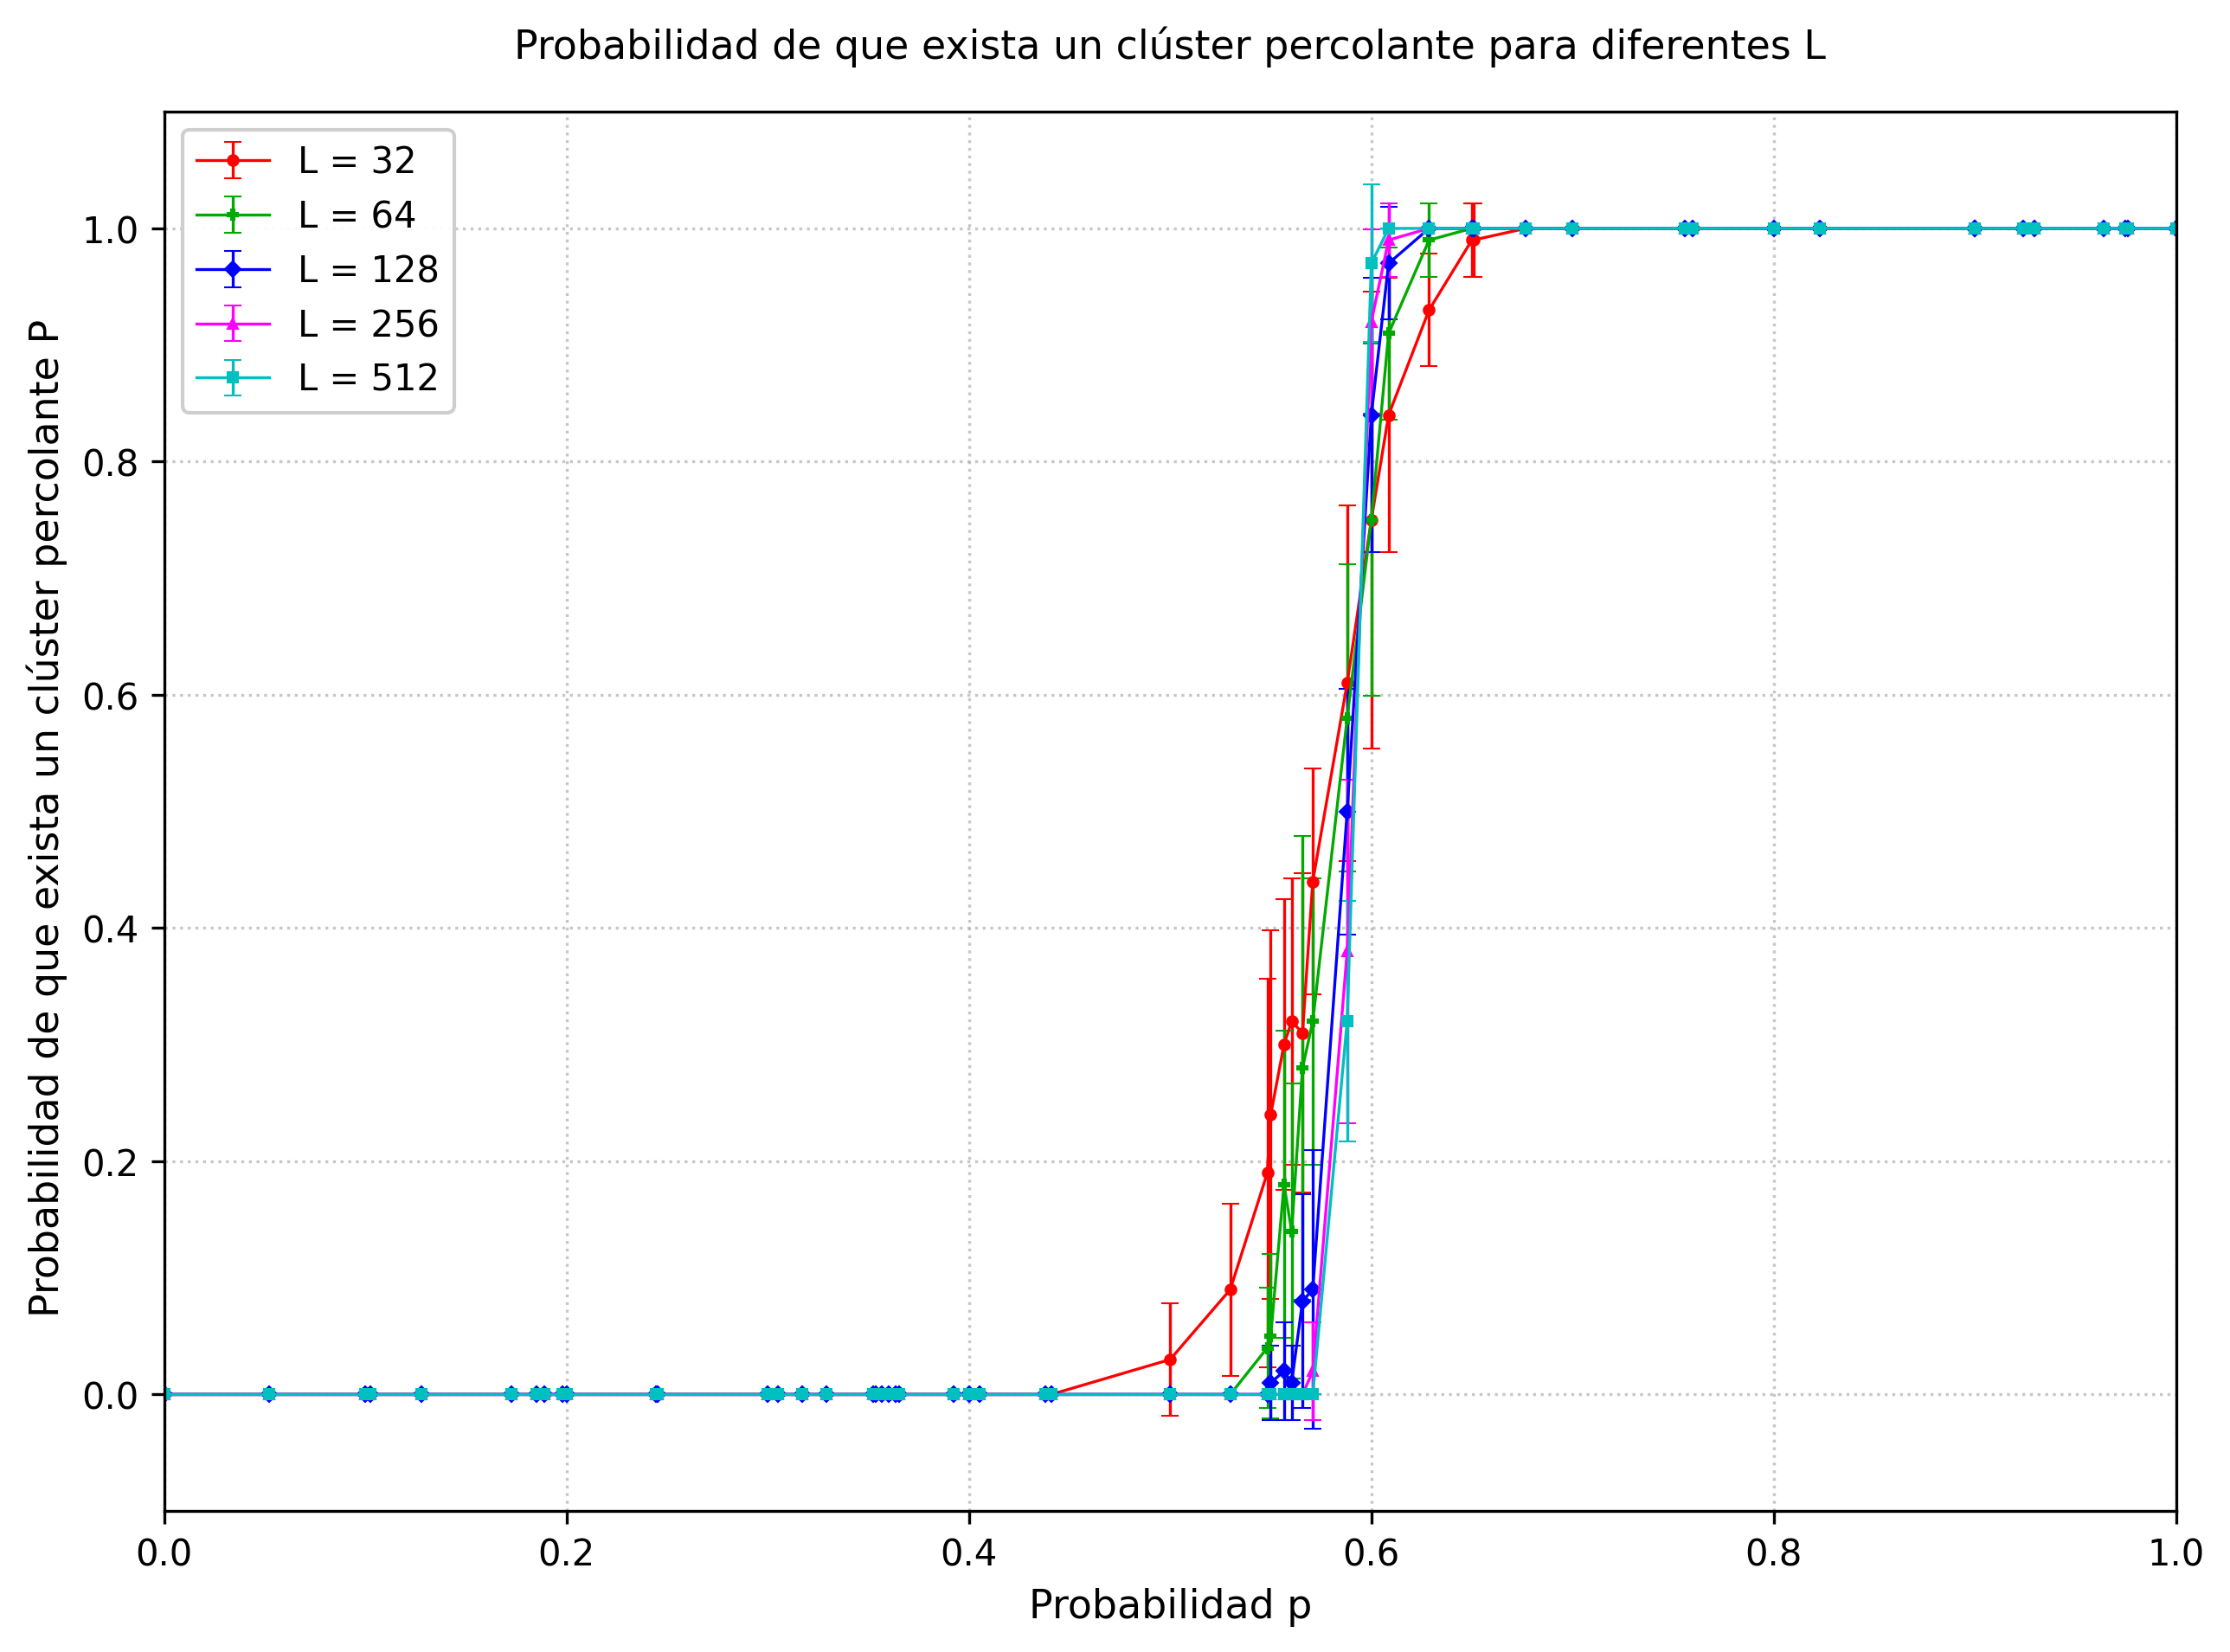
\includegraphics[width=1.0\linewidth]{../figures/P_all_L.png}
   \caption{Probabilidad de percolación en función de la probabilidad de llenado para distintos L.}
    \label{fig:5}
\end{figure}

Como se puede observar, $P(p,L)$ se aproxima a una función de Heaviside $\Theta(p-p_c)$ para $L\rightarrow\infty$, tal que $p_c\approx$ 5.9, es decir, el limite termodinámico. También, se observa que las incertidumbres son mayores en la vecindad de $p_C$, lo cual es esperable porque cerca del punto crítico las fluctuaciones son más intensas.
\\

En ese sentido, es posible observar la transición de fase del sistema entre $p\in$(0.55, 0.62) al pasar $P(p<p_C,L)$ = 0 a $P(p>p_C,L)$ = 1. Sin embargo, el comportamiento en general para $P(p,L)$ varia según la dimensión del sistema $L$ cerca de $p_c$, a este fenómeno se le conoce como escalamiento crítico.

\subsection{Tamaño promedio del clúster percolante mas grande $s(p,L)$}

Los resultados obtenidos para el tamaño medio de clúster de percolación $s(p,L)$ por medio del script en $\texttt{bash}$ son presentados en la figura \ref{fig:6}.

\begin{figure}[H]
   \centering
   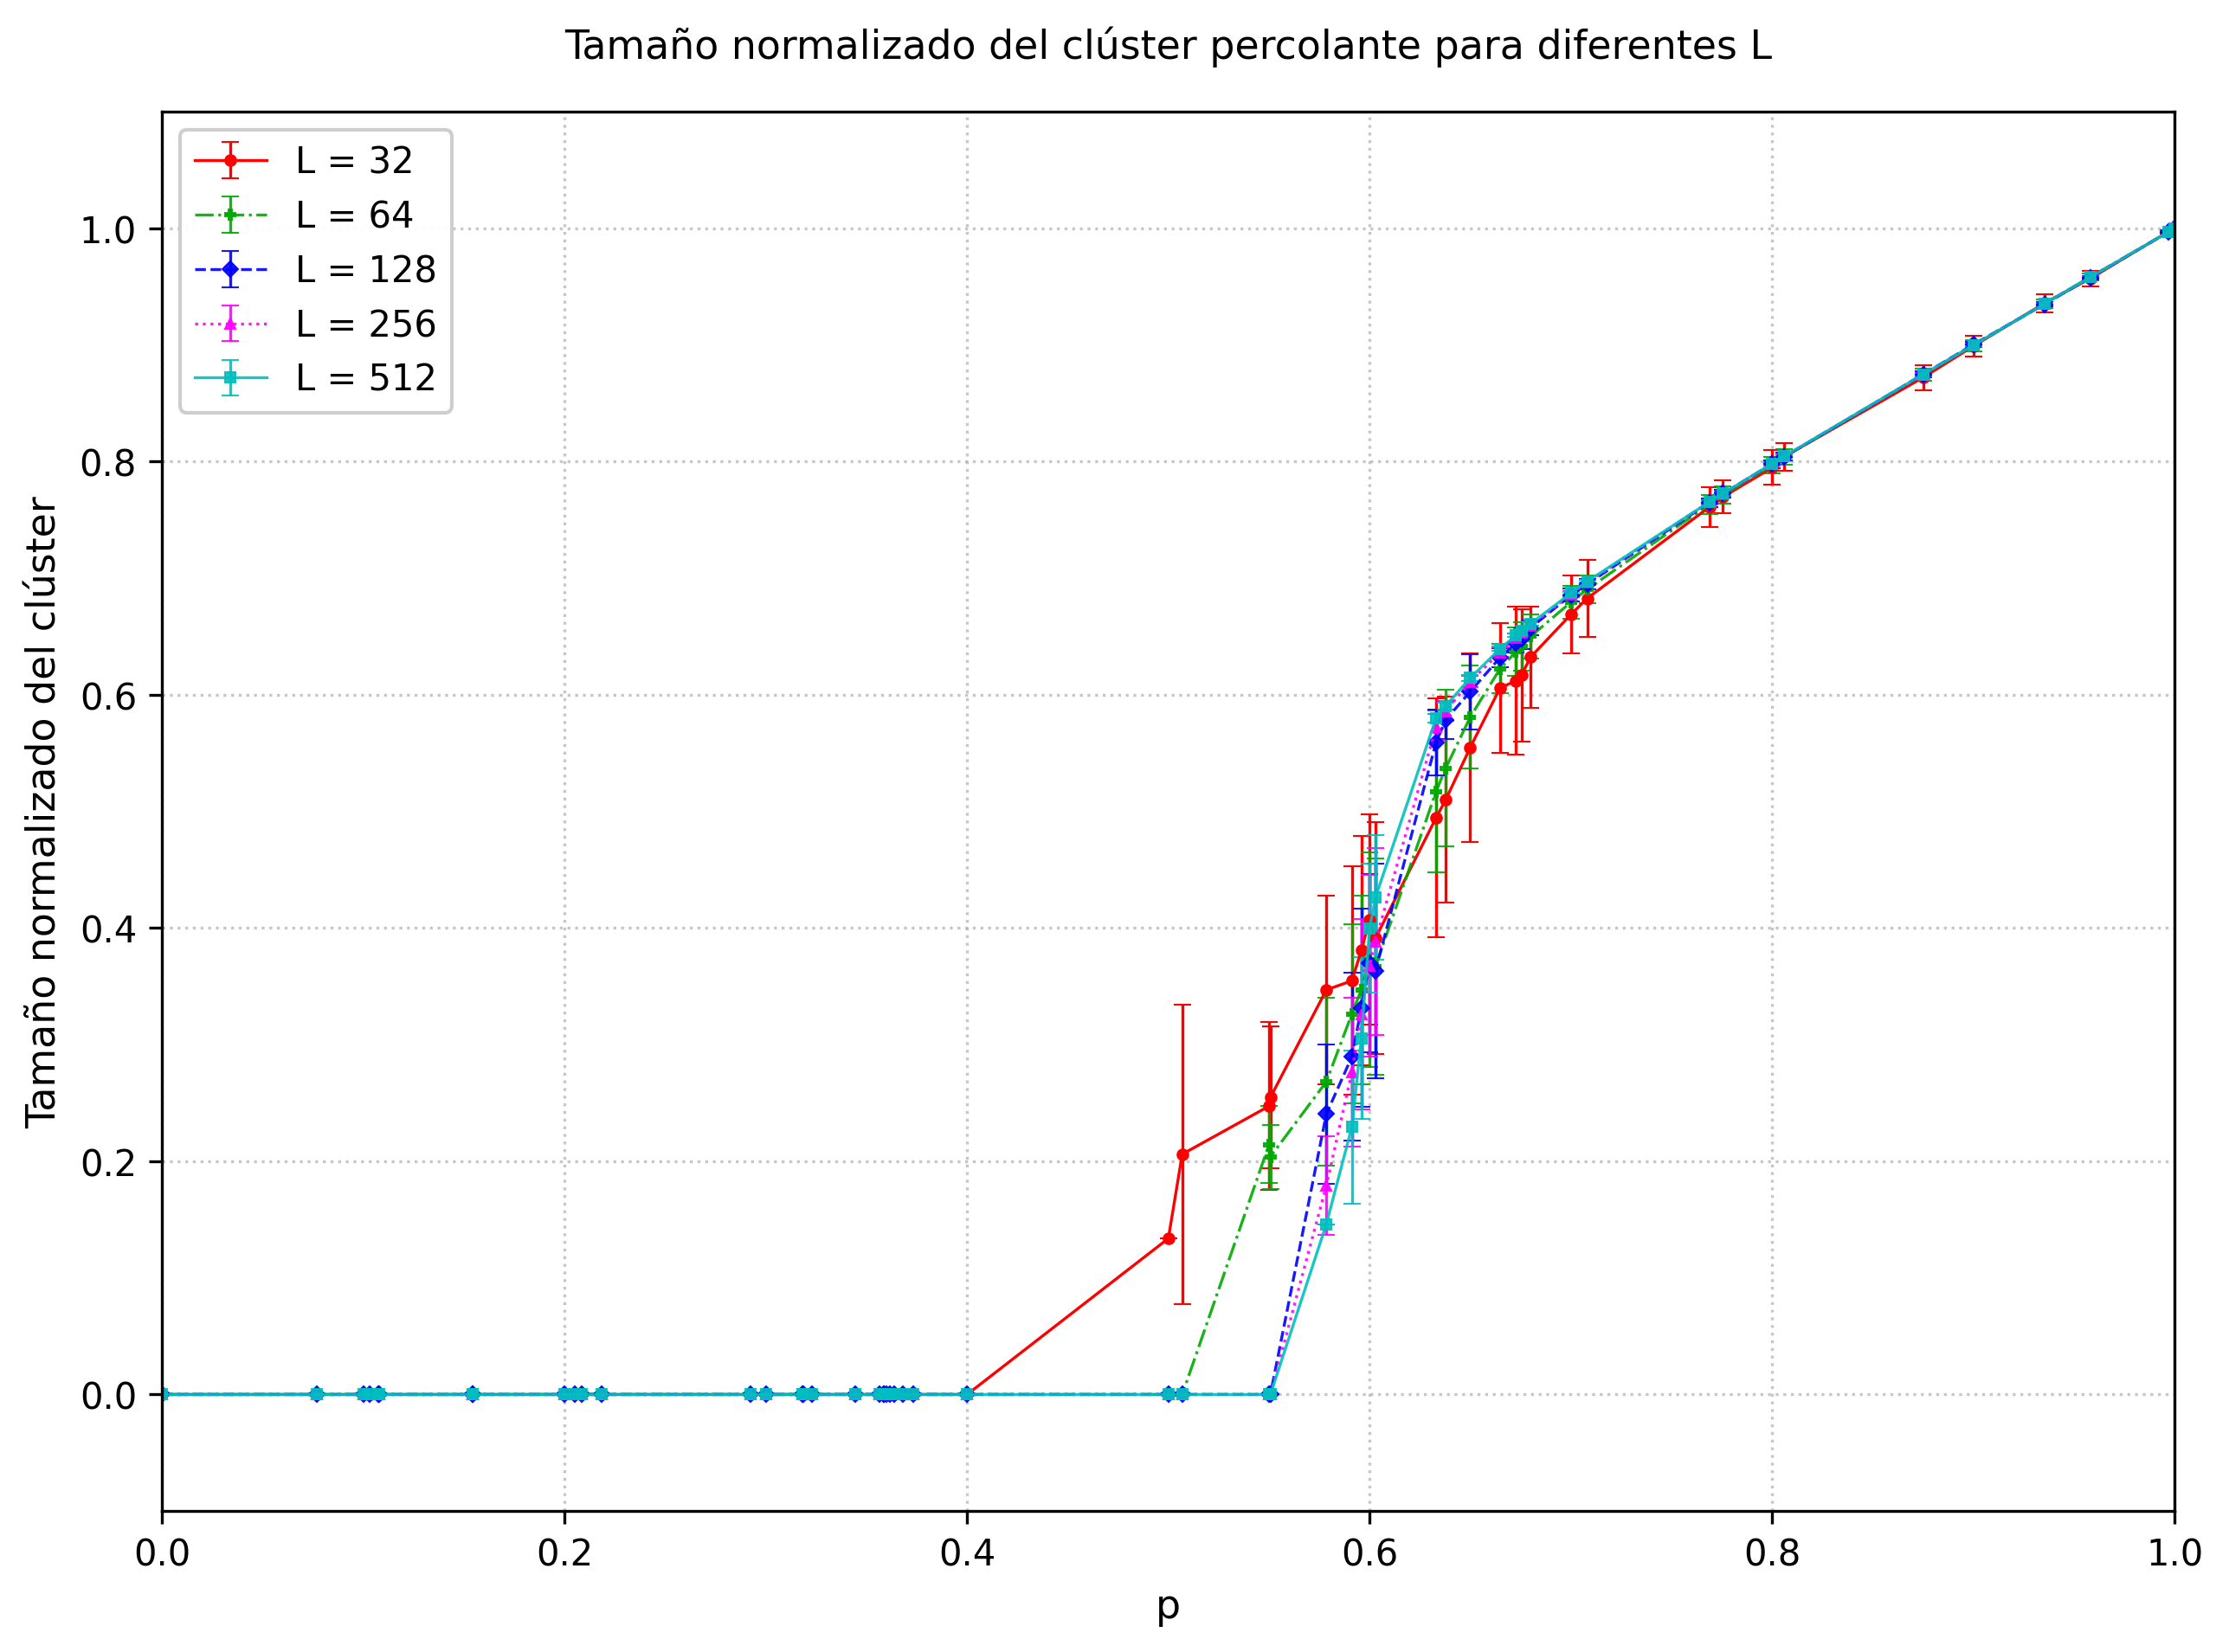
\includegraphics[width=1.0\linewidth]{../figures/Cluster_all_L.png}
    \caption{Tamaño medio de clúster de percolación en función de la probabilidad de llenado para distintos L.}
    \label{fig:6}
\end{figure}

Como se puede observar, $s(p,L)$ se observa una tendencia en su comportamiento para $L\rightarrow\infty$ de converger a una misma solución, la cual es distinta de cero cerca de la probabilidad critica $p_c\approx$ 5.9. 

\section{Conclusiones}

El estudio realizado permitió caracterizar satisfactoriamente el fenómeno de percolación en redes bidimensionales mediante simulaciones computacionales. Los principales hallazgos y conclusiones son:

\begin{itemize}
    \item Se confirmó el comportamiento crítico del sistema alrededor de $p_c \approx 0.5927$, donde la probabilidad de percolación $P(p,L)$ muestra una transición abrupta al aumentar el tamaño de la red $L$, aproximándose a una función escalón en el límite termodinámico, $L \rightarrow \infty$.

    \item El algoritmo de Hoshen-Kopelman demostró ser eficiente para el análisis de sistemas de tamaño moderado, $L \leq 2000$, aunque el análisis de profiling reveló que aproximadamente el 78\% del tiempo de ejecución se concentra en solo dos funciones: la identificación de clústeres (55\%) y la generación de la matriz aleatoria (23\%).

    \item Las optimizaciones implementadas, $\texttt{-O1}$ y $\texttt{-O3}$, mostraron mejoras modestas en el tiempo de ejecución, sugiriendo que el algoritmo ya está altamente optimizado en su forma básica. Los intentos de optimización manual adicional no produjeron mejoras significativas.

    \item Las simulaciones para diferentes tamaños de red permitieron observar el fenómeno de escalamiento crítico, donde las propiedades del sistema cerca de $p_c$ dependen fuertemente del tamaño $L$, mientras que lejos del punto crítico el comportamiento es más universal.

    \item La implementación modular y el uso de herramientas modernas ($\texttt{GNU Parallel, perf, Catch2}$) demostraron ser efectivos para manejar la naturaleza intensiva en cómputo de las simulaciones, permitiendo la generación de resultados estadísticamente robustos.
\end{itemize}

\section{Apéndice}

\subsection{Uso de herramientas externas: Todoist}
Para la realización de este proyecto se utilizo Todoist para coordinar y gestionar el trabajo entre los miembros del grupo. Se adjunta evidencia gráfica en la figura \ref{fig:7}.

\begin{figure}[H]
    \centering
    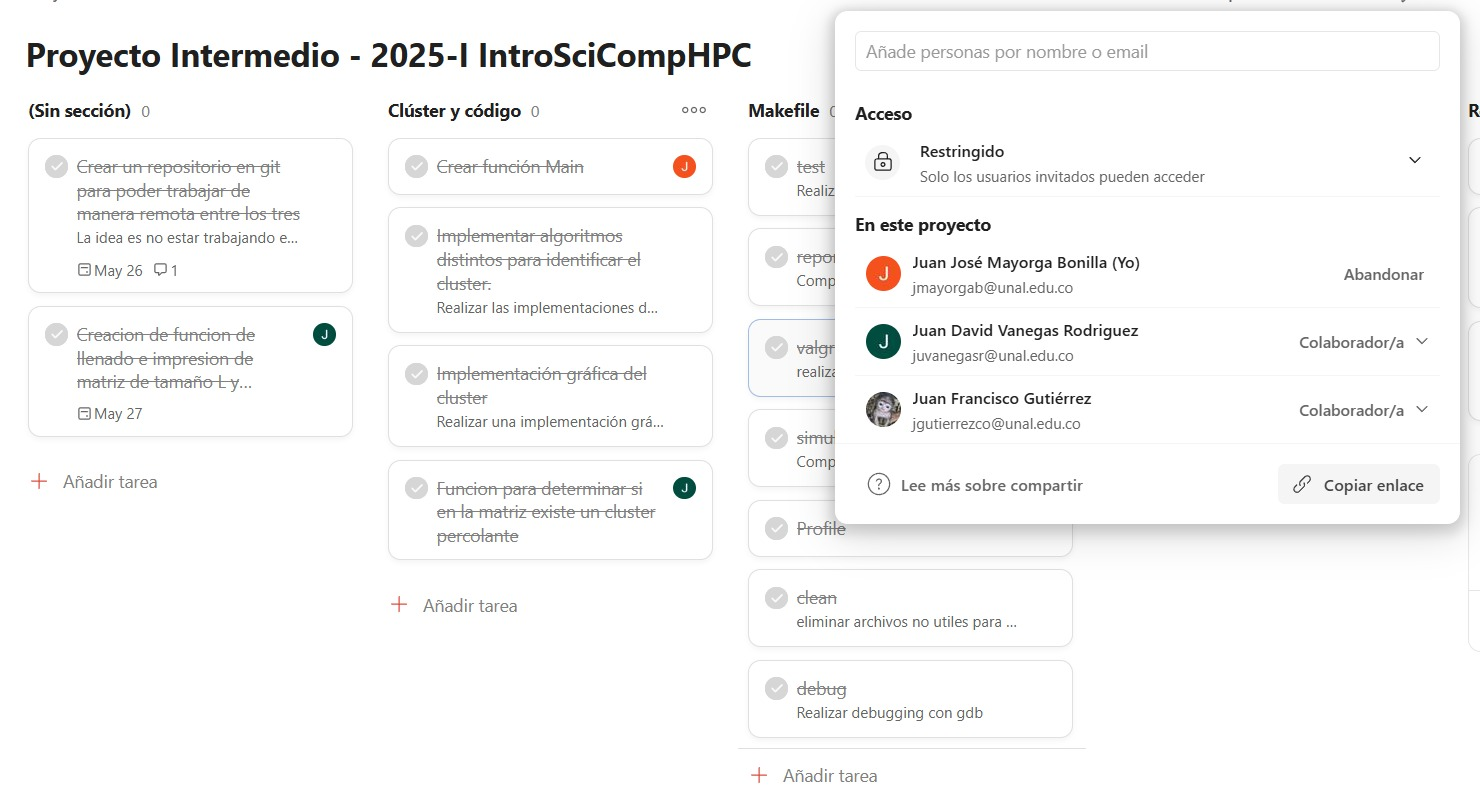
\includegraphics[width=0.9\linewidth]{../figures/todoist.png}
    \caption{Gestión de tareas en Todoist.}
    \label{fig:7}
\end{figure}

\bibliographystyle{plain}
\bibliography{report}



\end{document}